\subsection{Continuous Dynamics}
\logToConsole{EXAMPLES: CONTINUOUS DYNAMICS}

This section presents a variety of examples for continuous dynamics categorized along the different classes for dynamic systems realized in CORA. All subsequent examples can handle uncertain inputs. Uncertain parameters can be realized using different techniques:
\begin{enumerate}
    \item Introduce constant parameters as additional states and assign the dynamics $\dot{x}_i = 0$ to them. The disadvantage is that the dimension of the system is growing.
    \item Introduce time-varying parameters as additional uncertain inputs.
    \item Use specialized functions in CORA that can handle uncertain parameters.
\end{enumerate}
It is generally advised to use the last technique, but there is no proof that this technique always provides better results compared to the other techniques.

\subsubsection{Linear Dynamics}

For linear dynamics we demonstrate the usage of two different reachability algorithms.

\paragraph{Standard Algorithm}

First, we consider the standard algorithm from \cite{Girard2005}. We use a simple academic example from \cite[Sec.~3.2.3]{Althoff2010a} with not much focus on a connection to a real system. However, since linear systems are solely determined by their state and input matrix, adjusting this example to any other linear system is straightforward. Here, the system dynamics is
\begin{equation*}
    \dot{x}=\begin{bmatrix}
                -1 & -4 & 0  & 0  & 0  \\
                4  & -1 & 0  & 0  & 0  \\
                0  & 0  & -3 & 1  & 0  \\
                0  & 0  & -1 & -3 & 0  \\
                0  & 0  & 0  & 0  & -2 \\
    \end{bmatrix}  x + u(t), \quad
    x(0)\in\begin{bmatrix} [0.9,1.1]
               \\ [0.9,1.1] \\ [0.9,1.1] \\ [0.9,1.1] \\ [0.9,1.1]
    \end{bmatrix}, \,
    u(t) \in
    \begin{bmatrix}
    [0.9,1.1]
        \\
        [-0.25,0.25] \\
        [-0.1,0.1] \\
        [0.25,0.75] \\
        [-0.75,-0.25] \\
    \end{bmatrix}.
\end{equation*}

The MATLAB code that implements the simulation and reachability analysis of the linear example is (see file \textit{examples/contDynamics/linearSys/example\_linear\_reach\_01\_5dim.m} in the CORA toolbox):
    {\small
% This file was automatically created from the m-file 
% "m2tex.m" written by USL. 
% The fontencoding in this file is UTF-8. 
%  
% You will need to include the following two packages in 
% your LaTeX-Main-File. 
%  
% \usepackage{color} 
% \usepackage{fancyvrb} 
%  
% It is advised to use the following option for Inputenc 
% \usepackage[utf8]{inputenc} 
%  
  
% definition of matlab colors: 
\definecolor{mblue}{rgb}{0,0,1} 
\definecolor{mgreen}{rgb}{0.13333,0.5451,0.13333} 
\definecolor{mred}{rgb}{0.62745,0.12549,0.94118} 
\definecolor{mgrey}{rgb}{0.5,0.5,0.5} 
\definecolor{mdarkgrey}{rgb}{0.25,0.25,0.25} 
  
\DefineShortVerb[fontfamily=courier,fontseries=m]{\$} 
\DefineShortVerb[fontfamily=courier,fontseries=b]{\#} 
  
\noindent                                                                
 $$\color{mgreen}$% Parameter ---------------------------------------------------------------$\color{black}$$\\
 $$\\
 $params.tFinal = 5;$\\
 $params.R0 = zonotope([ones(5,1),0.1*diag(ones(5,1))]);$\\
 $params.U = zonotope(interval([0.9; -0.25; -0.1; 0.25; -0.75],$\color{mblue}$ ...$\color{black}$$\\
 $                             [1.1; 0.25; 0.1; 0.75; -0.25]));$\\
 $$\\
 $$\\
 $$\color{mgreen}$% Reachability Settings ---------------------------------------------------$\color{black}$$\\
 $$\\
 $options.timeStep = 0.02; $\\
 $options.taylorTerms = 4;$\\
 $options.zonotopeOrder = 20; $\\
 $$\\
 $$\\
 $$\color{mgreen}$% System Dynamics ---------------------------------------------------------$\color{black}$$\\
 $$\\
 $A = [-1 -4 0 0 0; 4 -1 0 0 0; 0 0 -3 1 0; 0 0 -1 -3 0; 0 0 0 0 -2];$\\
 $B = 1;$\\
 $$\\
 $fiveDimSys = linearSys($\color{mred}$'fiveDimSys'$\color{black}$,A,B);$\\
 $$\\
 $$\\
 $$\color{mgreen}$% Reachability Analysis ---------------------------------------------------$\color{black}$$\\
 $$\\
 $tic$\\
 $R = reach(fiveDimSys, params, options);$\\
 $tComp = toc;$\\
 $disp([$\color{mred}$'computation time of reachable set: '$\color{black}$,num2str(tComp)]);$\\
 $$\\
 $$\\
 $$\color{mgreen}$% Simulation --------------------------------------------------------------$\color{black}$$\\
 $$\\
 $simOpt.points = 25;$\\
 $simOpt.fracVert = 0.5;$\\
 $simOpt.fracInpVert = 0.5;$\\
 $simOpt.nrConstInp = 10;$\\
 $$\\
 $simRes = simulateRandom(fiveDimSys, params, simOpt);$\\
 $$\\
 $$\\
 $$\color{mgreen}$% Visualization -----------------------------------------------------------$\color{black}$$\\
 $$\\
 $$\color{mgreen}$% plot different projections$\color{black}$$\\
 $dims = {[1 2],[3 4]};$\\
 $$\\
 $$\color{mblue}$for$\color{black}$ k = 1:length(dims)$\\
 $    $\\
 $    figure; hold $\color{mred}$on$\color{black}$$\\
 $    projDims = dims{k};$\\
 $$\\
 $    $\color{mgreen}$% plot reachable sets $\color{black}$$\\
 $    plot(R,projDims,$\color{mred}$'FaceColor'$\color{black}$,[.8 .8 .8],$\color{mred}$'EdgeColor'$\color{black}$,$\color{mred}$'b'$\color{black}$);$\\
 $    $\\
 $    $\color{mgreen}$% plot initial set$\color{black}$$\\
 $    plot(params.R0,projDims,$\color{mred}$'w-'$\color{black}$,$\color{mred}$'lineWidth'$\color{black}$,2);$\\
 $    $\\
 $    $\color{mgreen}$% plot simulation results$\color{black}$$\\
 $    plot(simRes,projDims,$\color{mred}$'y'$\color{black}$);$\\
 $$\\
 $    $\color{mgreen}$% label plot$\color{black}$$\\
 $    xlabel([$\color{mred}$'x_{'$\color{black}$,num2str(projDims(1)),$\color{mred}$'}'$\color{black}$]);$\\
 $    ylabel([$\color{mred}$'x_{'$\color{black}$,num2str(projDims(2)),$\color{mred}$'}'$\color{black}$]);$\\
 $$\color{mblue}$end$\color{black}$$\\ 
  
\UndefineShortVerb{\$} 
\UndefineShortVerb{\#}}

The reachable set and the simulation are plotted in \cref{fig:example_linear_reach_01_5dim} for a time horizon of $t_f = 5$.

\begin{figure}[htb]
    \centering
    \footnotesize
    \includetikz{./figures/tikz/examples/contDynamics/example_linear_reach_01_5dim}
    \caption{Illustration of the reachable set of the linear example. The white box shows the initial set and the black lines show simulated trajectories.}
    \label{fig:example_linear_reach_01_5dim}
\end{figure}

\paragraph{Adaptive Algorithm}

One major disadvantage of the standard algorithm used in the example above is that the user is required to manually tune the time step size, the number of Taylor terms, and the zonotope order to obtain a tight enclosure of the reachable set. The novel adaptive algorithm from \cite{Wetzlinger2020} tunes these parameters automatically in such a way that a certain precision is achieved. We consider the two-dimensional system
\begin{equation*}
    \dot{x}=\begin{bmatrix}
                -0.7 & -2 \\ 2 & -0.7
    \end{bmatrix}  x + u(t), \quad
    x(0)\in\begin{bmatrix} [9.5,10.5]
               \\ [4.5,5.5]
    \end{bmatrix}, \,
    u(t) \in
    \begin{bmatrix}
    [0.75,1.25]
        \\
        [0.75,1.25] \\
    \end{bmatrix}.
\end{equation*}

The MATLAB code that implements reachability analysis with the adaptive algorithm (see file \textit{examples/contDynamics/linearSys/example\_linear\_reach\_04\_adaptive.m} in the CORA toolbox):
    {\small
% This file was automatically created from the m-file 
% "m2tex.m" written by USL. 
% The fontencoding in this file is UTF-8. 
%  
% You will need to include the following two packages in 
% your LaTeX-Main-File. 
%  
% \usepackage{color} 
% \usepackage{fancyvrb} 
%  
% It is advised to use the following option for Inputenc 
% \usepackage[utf8]{inputenc} 
%  
  
% definition of matlab colors: 
\definecolor{mblue}{rgb}{0,0,1} 
\definecolor{mgreen}{rgb}{0.13333,0.5451,0.13333} 
\definecolor{mred}{rgb}{0.62745,0.12549,0.94118} 
\definecolor{mgrey}{rgb}{0.5,0.5,0.5} 
\definecolor{mdarkgrey}{rgb}{0.25,0.25,0.25} 
  
\DefineShortVerb[fontfamily=courier,fontseries=m]{\$} 
\DefineShortVerb[fontfamily=courier,fontseries=b]{\#} 
  
\noindent                                                                         
 $$\color{mgreen}$% System Dynamics ---------------------------------------------------------$\color{black}$$\\
 $$\\
 $A = [-0.7 -2; 2 -0.7];$\\
 $B = 1;$\\
 $$\\
 $sys = linearSys($\color{mred}$'sys'$\color{black}$,A,B);$\\
 $$\\
 $$\\
 $$\color{mgreen}$% Parameter ---------------------------------------------------------------$\color{black}$$\\
 $$\\
 $dim = length(A);$\\
 $$\\
 $params.tFinal = 5;$\\
 $params.R0 = zonotope([[10; 5],0.5*eye(dim)]);       $\color{mgreen}$% initial set$\color{black}$$\\
 $params.U = zonotope([ones(dim,1),0.25*eye(dim)]);   $\color{mgreen}$% uncertain inputs$\color{black}$$\\
 $$\\
 $$\\
 $$\color{mgreen}$% Reachability Settings ---------------------------------------------------$\color{black}$$\\
 $$\\
 $options.linAlg = $\color{mred}$'adaptive'$\color{black}$; $\color{mgreen}$% adaptive parameter tuning$\color{black}$$\\
 $$\\
 $$\\
 $$\color{mgreen}$% Simulation --------------------------------------------------------------$\color{black}$$\\
 $$\\
 $simOpt.points = 10;$\\
 $simOpt.fracVert = 0.5;$\\
 $simOpt.fracInpVert = 0.5;$\\
 $simOpt.nrConstInp = 10;$\\
 $$\\
 $simRes = simulateRandom(sys, params, simOpt);$\\
 $$\\
 $$\\
 $$\color{mgreen}$% Reachability Analysis ---------------------------------------------------$\color{black}$$\\
 $$\\
 $errs = [1;0.05];$\\
 $stepssS = zeros(length(errs),1);$\\
 $timesS = zeros(length(errs),1);$\\
 $R = cell(length(errs),1);$\\
 $$\\
 $$\color{mgreen}$% compute reachable sets for different max. allowed errors$\color{black}$$\\
 $$\color{mblue}$for$\color{black}$ i=1:length(errs)$\\
 $    options.error = errs(i);$\\
 $    tic$\\
 $    R{i} = reach(sys,params,options);$\\
 $    timesS(i) = toc;$\\
 $    stepssS(i) = length(R{i}.timeInterval.set);$\\
 $$\color{mblue}$end$\color{black}$$\\
 $$\\
 $$\\
 $$\color{mgreen}$% Visualization -----------------------------------------------------------$\color{black}$$\\
 $$\\
 $figure; hold $\color{mred}$on$\color{black}$; box $\color{mred}$on$\color{black}$;$\\
 $projDims = [1,2];$\\
 $$\\
 $$\color{mgreen}$% plot reachable set$\color{black}$$\\
 $plot(R{1},projDims,$\color{mred}$$\color{mred}$'k'$\color{black}$$\color{black}$,$\color{mred}$'EdgeColor'$\color{black}$,$\color{mred}$$\color{mred}$'k'$\color{black}$$\color{black}$);$\\
 $plot(R{2},projDims,$\color{mred}$'FaceColor'$\color{black}$,[0.7,0.7,0.7],$\color{mred}$'EdgeColor'$\color{black}$,[0.7,0.7,0.7]);$\\
 $$\\
 $$\color{mgreen}$% plot initial set$\color{black}$$\\
 $plot(params.R0,projDims,$\color{mred}$'w'$\color{black}$,$\color{mred}$'LineWidth'$\color{black}$,1.5);$\\
 $$\\
 $$\color{mgreen}$% plot simulation$\color{black}$$\\
 $plot(simRes,projDims,$\color{mred}$'b'$\color{black}$,$\color{mred}$'LineWidth'$\color{black}$,0.5);$\\
 $$\\
 $$\color{mgreen}$% plot unsafe set$\color{black}$$\\
 $unsafeSet = interval([2;-2],[4;2]);$\\
 $plot(unsafeSet,projDims,$\color{mred}$'FaceColor'$\color{black}$,[227,114,34]/255,...$\\
 $    $\color{mred}$'EdgeColor'$\color{black}$,$\color{mred}$'r'$\color{black}$,$\color{mred}$'LineWidth'$\color{black}$,2);$\\
 $$\\
 $$\color{mgreen}$% formatting$\color{black}$$\\
 $xlabel($\color{mred}$'x_1'$\color{black}$); ylabel($\color{mred}$'x_2'$\color{black}$);$\\
 $title($\color{mred}$'2D system'$\color{black}$);$\\
 $             $\\ 
  
\UndefineShortVerb{\$} 
\UndefineShortVerb{\#}}

The reachable sets computed with the adaptive algorithm for two different precision values are plotted in \cref{fig:example_linear_reach_04_adaptive} for a time horizon of $t_f = 5$.

\begin{figure}[htb]
    \centering
    \footnotesize
    \includetikz{./figures/tikz/examples/contDynamics/example_linear_reach_04_adaptive}
    \caption{Illustration of the reachable set computed with the adaptive algorithm with a requested precision of \texttt{options.error = 1} (black) and \texttt{options.error = 0.05} (gray).}
    \label{fig:example_linear_reach_04_adaptive}
\end{figure}

\subsubsection{Linear Dynamics with Uncertain Parameters}

For linear dynamics with uncertain parameters, we use the transmission line example from \cite[Sec.~4.5.2]{Althoff2011b}, which can be modeled as an electric circuit with resistors, inductors, and capacitors. The parameters of each component have uncertain values as described in \cite[Sec.~4.5.2]{Althoff2011b}. This example shows how one can better take care of dependencies of parameters by using matrix zonotopes instead of interval matrices.

The MATLAB code that implements the simulation and reachability analysis of the linear example with uncertain parameters is (see file \textit{examples/contDynamics/linParamSys/}\\ \textit{example\_linearParam\_reach\_01\_rlc\_const.m} in the CORA toolbox):
    {\small
% This file was automatically created from the m-file 
% "m2tex.m" written by USL. 
% The fontencoding in this file is UTF-8. 
%  
% You will need to include the following two packages in 
% your LaTeX-Main-File. 
%  
% \usepackage{color} 
% \usepackage{fancyvrb} 
%  
% It is advised to use the following option for Inputenc 
% \usepackage[utf8]{inputenc} 
%  
  
% definition of matlab colors: 
\definecolor{mblue}{rgb}{0,0,1} 
\definecolor{mgreen}{rgb}{0.13333,0.5451,0.13333} 
\definecolor{mred}{rgb}{0.62745,0.12549,0.94118} 
\definecolor{mgrey}{rgb}{0.5,0.5,0.5} 
\definecolor{mdarkgrey}{rgb}{0.25,0.25,0.25} 
  
\DefineShortVerb[fontfamily=courier,fontseries=m]{\$} 
\DefineShortVerb[fontfamily=courier,fontseries=b]{\#} 
  
\noindent                                                                                                             
 $$\color{mgreen}$% System Dynamics ---------------------------------------------------------$\color{black}$$\\
 $$\\
 $$\color{mgreen}$% get matrix zonotopes of the model$\color{black}$$\\
 $[matZ_A,matZ_B] = RLCcircuit();$\\
 $matI_A = intervalMatrix(matZ_A);$\\
 $dim = matZ_A.dim;$\\
 $$\\
 $$\color{mgreen}$% create linear parametric systems with constant parameters$\color{black}$$\\
 $sysMatZono  = linParamSys(matZ_A, eye(dim));$\\
 $sysIntMat = linParamSys(matI_A, eye(dim));$\\
 $$\\
 $$\\
 $$\color{mgreen}$% Parameter ---------------------------------------------------------------$\color{black}$$\\
 $$\\
 $$\color{mgreen}$% compute initial set$\color{black}$$\\
 $u0 = intervalMatrix(0,0.2);             $\color{mgreen}$% range of voltages$\color{black}$$\\
 $$\\
 $intA = intervalMatrix(matZ_A);$\\
 $invAmid = inv(center(intA.int));        $\color{mgreen}$% inverse of A$\color{black}$$\\
 $$\\
 $intB = intervalMatrix(matZ_B);$\\
 $R0 = invAmid*intB*u0 + intervalMatrix(0,1e-3*ones(dim,1));$\\
 $$\\
 $params.R0 = zonotope(interval(R0));     $\color{mgreen}$% convert initial set to zonotope$\color{black}$$\\
 $$\\
 $$\color{mgreen}$% uncertain inputs$\color{black}$$\\
 $u = intervalMatrix(1,0.01);$\\
 $params.U = zonotope(interval(intB*u));$\\
 $$\\
 $$\color{mgreen}$% final time$\color{black}$$\\
 $params.tFinal = 0.3;$\\
 $$\\
 $$\\
 $$\color{mgreen}$% Reachability Settings ---------------------------------------------------$\color{black}$$\\
 $$\\
 $options.intermediateOrder = 2;$\\
 $options.timeStep = 0.001;$\\
 $options.zonotopeOrder = 400;$\\
 $options.taylorTerms = 8;$\\
 $options.compTimePoint = false;$\\
 $$\\
 $$\\
 $$\color{mgreen}$% Reachability Analysis ---------------------------------------------------$\color{black}$$\\
 $$\\
 $$\color{mgreen}$% compute reachable set using matrix zonotopes$\color{black}$$\\
 $tic$\\
 $RmatZono = reach(sysMatZono, params, options);$\\
 $tComp = toc;$\\
 $disp([$\color{mred}$'computation time (matrix zonotopes): '$\color{black}$,num2str(tComp)]);$\\
 $$\\
 $$\color{mgreen}$% compute reachable set using interval matrices$\color{black}$$\\
 $tic$\\
 $RintMat = reach(sysIntMat, params, options);$\\
 $tComp = toc;$\\
 $disp([$\color{mred}$'computation time (interval matrices): '$\color{black}$,num2str(tComp)]);$\\
 $$\\
 $$\\
 $$\color{mgreen}$% Simulation --------------------------------------------------------------$\color{black}$$\\
 $$\\
 $simOpt.points = 60;$\\
 $simOpt.fracVert = 0.5;$\\
 $simOpt.fracInpVert = 0.5;$\\
 $simOpt.nrConstInp = 6;$\\
 $$\\
 $simRes = simulateRandom(sysIntMat, params, simOpt);$\\
 $$\\
 $$\\
 $$\color{mgreen}$% Visualization -----------------------------------------------------------$\color{black}$$\\
 $$\\
 $$\color{mgreen}$% PLOT 1: state space$\color{black}$$\\
 $$\\
 $figure; $\\
 $hold $\color{mred}$on$\color{black}$$\\
 $projDim = [20,40];$\\
 $    $\\
 $$\color{mgreen}$% plot reachable sets$\color{black}$$\\
 $hanIntMat = plot(RintMat,projDim,$\color{mred}$'FaceColor'$\color{black}$,[.6 .6 .6],$\color{mred}$'Order'$\color{black}$,10);$\\
 $hanMatZono = plot(RmatZono,projDim,$\color{mred}$'FaceColor'$\color{black}$,[.8 .8 .8],$\color{mred}$'Order'$\color{black}$,10);$\\
 $$\\
 $$\color{mgreen}$% plot initial set$\color{black}$$\\
 $plot(params.R0,projDim,$\color{mred}$'k'$\color{black}$,$\color{mred}$'FaceColor'$\color{black}$,$\color{mred}$'k'$\color{black}$);$\\
 $$\\
 $$\color{mgreen}$% plot simulation results     $\color{black}$$\\
 $plot(simRes,projDim);$\\
 $$\\
 $$\color{mgreen}$% label plot$\color{black}$$\\
 $xlabel([$\color{mred}$'x_{'$\color{black}$,num2str(projDim(1)),$\color{mred}$'}'$\color{black}$]);$\\
 $ylabel([$\color{mred}$'x_{'$\color{black}$,num2str(projDim(2)),$\color{mred}$'}'$\color{black}$]);$\\
 $legend([hanIntMat,hanMatZono],$\color{mred}$'Interval matrix'$\color{black}$,$\color{mred}$'Matrix zonotope'$\color{black}$);$\\
 $$\\
 $$\\
 $$\color{mgreen}$% PLOT 2: reachable set over time$\color{black}$$\\
 $$\\
 $figure; $\\
 $hold $\color{mred}$on$\color{black}$$\\
 $$\\
 $$\color{mgreen}$% plot time elapse$\color{black}$$\\
 $hanIntMat = plotOverTime(RintMat,0.5*dim,$\color{mred}$'FaceColor'$\color{black}$,[.6 .6 .6]);$\\
 $hanMatZono = plotOverTime(RmatZono,0.5*dim,$\color{mred}$'FaceColor'$\color{black}$,[.8 .8 .8]);$\\
 $$\\
 $$\color{mgreen}$% plot simulation results$\color{black}$$\\
 $plotOverTime(simRes,0.5*dim);$\\
 $$\\
 $$\color{mgreen}$% label plot$\color{black}$$\\
 $xlabel($\color{mred}$'t'$\color{black}$);$\\
 $ylabel([$\color{mred}$'x_{'$\color{black}$,num2str(0.5*dim),$\color{mred}$'}'$\color{black}$]);$\\
 $legend([hanIntMat,hanMatZono],$\color{mred}$'Interval matrix'$\color{black}$,$\color{mred}$'Matrix zonotope'$\color{black}$);$\\ 
  
\UndefineShortVerb{\$} 
\UndefineShortVerb{\#}}

The reachable set and the simulation are plotted in \cref{fig:example_linearParam_reach_01_rlc_const} for a time horizon of $t_f = 0.3$.
\begin{figure}[htb]
    \centering
    \footnotesize
    \includetikz{./figures/tikz/examples/contDynamics/example_linearParam_reach_01_rlc_const}
    \caption{Illustration of the reachable set of the transmission example. A white box shows the initial set and the black lines are simulated trajectories.}
    \label{fig:example_linearParam_reach_01_rlc_const}
\end{figure}

\subsubsection{Nonlinear Dynamics}

For nonlinear dynamics, several examples are presented.

\paragraph{Tank System}
The first example is the tank system from \cite{Althoff2008c} where water flows from one tank into another one. This example can be used to study the effect of water power plants on the water level of rivers. This example can be easy extended by several tanks and thus is a nice benchmark example to study the scalability of algorithms for reachability analysis. CORA can compute the reachable set with at least $100$ tanks.

The MATLAB code that implements the simulation and reachability analysis of the tank example is (see file \textit{examples/contDynamics/nonlinearSys/}\textit{example\_nonlinear\_reach\_01\_tank.m} in the CORA toolbox):
    {\small
% This file was automatically created from the m-file 
% "m2tex.m" written by USL. 
% The fontencoding in this file is UTF-8. 
%  
% You will need to include the following two packages in 
% your LaTeX-Main-File. 
%  
% \usepackage{color} 
% \usepackage{fancyvrb} 
%  
% It is advised to use the following option for Inputenc 
% \usepackage[utf8]{inputenc} 
%  
  
% definition of matlab colors: 
\definecolor{mblue}{rgb}{0,0,1} 
\definecolor{mgreen}{rgb}{0.13333,0.5451,0.13333} 
\definecolor{mred}{rgb}{0.62745,0.12549,0.94118} 
\definecolor{mgrey}{rgb}{0.5,0.5,0.5} 
\definecolor{mdarkgrey}{rgb}{0.25,0.25,0.25} 
  
\DefineShortVerb[fontfamily=courier,fontseries=m]{\$} 
\DefineShortVerb[fontfamily=courier,fontseries=b]{\#} 
  
\noindent                                                                
 $$\color{mgreen}$% Parameter ---------------------------------------------------------------$\color{black}$$\\
 $$\\
 $params.tFinal = 400;$\\
 $params.R0 = zonotope([[2; 4; 4; 2; 10; 4],0.2*eye(6)]);$\\
 $params.U = zonotope([0,0.005]);$\\
 $$\\
 $$\\
 $$\color{mgreen}$% Reachability Settings ---------------------------------------------------$\color{black}$$\\
 $$\\
 $options.timeStep = 1;$\\
 $options.taylorTerms = 4;$\\
 $options.zonotopeOrder = 50;$\\
 $$\\
 $options.intermediateOrder = 5;$\\
 $options.errorOrder = 1;$\\
 $options.alg = $\color{mred}$'lin'$\color{black}$;$\\
 $options.tensorOrder = 2;$\\
 $$\\
 $$\\
 $$\color{mgreen}$% System Dynamics ---------------------------------------------------------$\color{black}$$\\
 $$\\
 $tank = nonlinearSys(@tank6Eq);$\\
 $$\\
 $$\\
 $$\color{mgreen}$% Reachability Analysis ---------------------------------------------------$\color{black}$$\\
 $$\\
 $tic$\\
 $R = reach(tank, params, options);$\\
 $tComp = toc;$\\
 $disp([$\color{mred}$'computation time of reachable set: '$\color{black}$,num2str(tComp)]);$\\
 $$\\
 $$\\
 $$\color{mgreen}$% Simulation --------------------------------------------------------------$\color{black}$$\\
 $$\\
 $simOpt.points = 60;$\\
 $simOpt.fracVert = 0.5;$\\
 $simOpt.fracInpVert = 0.5;$\\
 $simOpt.nrConstInp = 6;$\\
 $$\\
 $simRes = simulateRandom(tank, params, simOpt);$\\
 $$\\
 $$\\
 $$\color{mgreen}$% Visualization -----------------------------------------------------------$\color{black}$$\\
 $$\\
 $dims = {[1 2],[3 4],[5 6]};$\\
 $$\\
 $$\color{mblue}$for$\color{black}$ k = 1:length(dims)$\\
 $    $\\
 $    figure; hold $\color{mred}$on$\color{black}$$\\
 $    projDim = dims{k};$\\
 $    $\\
 $    $\color{mgreen}$% plot reachable sets$\color{black}$$\\
 $    plot(R,projDim,$\color{mred}$'FaceColor'$\color{black}$,[.8 .8 .8]);$\\
 $    $\\
 $    $\color{mgreen}$% plot initial set$\color{black}$$\\
 $    plot(params.R0,projDim,$\color{mred}$'k'$\color{black}$,$\color{mred}$'FaceColor'$\color{black}$,$\color{mred}$'w'$\color{black}$);$\\
 $    $\\
 $    $\color{mgreen}$% plot simulation results     $\color{black}$$\\
 $    plot(simRes,projDim,$\color{mred}$'k'$\color{black}$);$\\
 $$\\
 $    $\color{mgreen}$% label plot$\color{black}$$\\
 $    xlabel([$\color{mred}$'x_{'$\color{black}$,num2str(projDim(1)),$\color{mred}$'}'$\color{black}$]);$\\
 $    ylabel([$\color{mred}$'x_{'$\color{black}$,num2str(projDim(2)),$\color{mred}$'}'$\color{black}$]);$\\
 $$\color{mblue}$end$\color{black}$$\\ 
  
\UndefineShortVerb{\$} 
\UndefineShortVerb{\#}}

The difference to specifying a linear system is that a link to a nonlinear differential equation has to be provided, rather than the system matrix $A$ and the input matrix $B$. The nonlinear system model $\dot{x}=f(x,u)$, where $x$ is the state and $u$ is the input, is shown below:
    {\small
% This file was automatically created from the m-file 
% "m2tex.m" written by USL. 
% The fontencoding in this file is UTF-8. 
%  
% You will need to include the following two packages in 
% your LaTeX-Main-File. 
%  
% \usepackage{color} 
% \usepackage{fancyvrb} 
%  
% It is advised to use the following option for Inputenc 
% \usepackage[utf8]{inputenc} 
%  
  
% definition of matlab colors: 
\definecolor{mblue}{rgb}{0,0,1} 
\definecolor{mgreen}{rgb}{0.13333,0.5451,0.13333} 
\definecolor{mred}{rgb}{0.62745,0.12549,0.94118} 
\definecolor{mgrey}{rgb}{0.5,0.5,0.5} 
\definecolor{mdarkgrey}{rgb}{0.25,0.25,0.25} 
  
\DefineShortVerb[fontfamily=courier,fontseries=m]{\$} 
\DefineShortVerb[fontfamily=courier,fontseries=b]{\#} 
  
\noindent              
 $$\color{mblue}$function$\color{black}$ dx = tank6Eq(x,u)$\\
 $$\\
 $    $\color{mgreen}$% parameter$\color{black}$$\\
 $    k = 0.015;$\\
 $    k2 = 0.01;$\\
 $    g = 9.81; $\\
 $$\\
 $    $\color{mgreen}$% differential equations$\color{black}$$\\
 $    dx(1,1) = u(1)+0.1+k2*(4-x(6))-k*sqrt(2*g)*sqrt(x(1));  $\color{mgreen}$% tank 1$\color{black}$$\\
 $    dx(2,1) = k*sqrt(2*g)*(sqrt(x(1))-sqrt(x(2)));          $\color{mgreen}$% tank 2$\color{black}$$\\
 $    dx(3,1) = k*sqrt(2*g)*(sqrt(x(2))-sqrt(x(3)));          $\color{mgreen}$% tank 3$\color{black}$$\\
 $    dx(4,1) = k*sqrt(2*g)*(sqrt(x(3))-sqrt(x(4)));          $\color{mgreen}$% tank 4$\color{black}$$\\
 $    dx(5,1) = k*sqrt(2*g)*(sqrt(x(4))-sqrt(x(5)));          $\color{mgreen}$% tank 5$\color{black}$$\\
 $    dx(6,1) = k*sqrt(2*g)*(sqrt(x(5))-sqrt(x(6)));          $\color{mgreen}$% tank 6$\color{black}$$\\ 
  
\UndefineShortVerb{\$} 
\UndefineShortVerb{\#}}

The output of this function is $\dot{x}$ for a given time $t$, state $x$, and input $u$.

\cref{fig:example_nonlinear_reach_01_tank} shows the reachable set and the simulation for a time horizon of $t_f = 400$.
\begin{figure}[htb]
    \centering
    \footnotesize
    \includetikz{./figures/tikz/examples/contDynamics/example_nonlinear_reach_01_tank}
    \caption{Illustration of the reachable set of the linear example. The white box shows the initial set and the black lines show simulated trajectories.}
    \label{fig:example_nonlinear_reach_01_tank}
\end{figure}

\paragraph{Van der Pol Oscillator}
The Van der Pol oscillator is a standard example for limit cycles. By using reachability analysis one can show that one always returns to the initial set so that the obtained set is an invariant set. This example is used in \cite{Althoff2008c} to demonstrate that one can obtain a solution even if the linearization error becomes too large by splitting the reachable set. Later, in \cite{Althoff2013a} an improved method is presented that requires less splitting. This example demonstrates the capabilities of the simpler approach presented in \cite{Althoff2008c}. Due to the similarity of the MATLAB code compared to the previous tank example, we only present the reachable set in \cref{fig:example_nonlinear_reach_03_vanderPol}. The corresponding code can be found in the file \textit{examples/contDynamics/nonlinearSys/}\textit{example\_nonlinear\_reach\_03\_vanDerPol\_splitting.m} in the CORA toolbox.
\begin{figure}[htb]
    \centering
    \footnotesize
    \includegraphics[width=0.5\columnwidth]{./figures/examples/example_nonlinear_reach_03_vanderPol.eps}
    \caption{Illustration of the reachable set of the Van der Pol oscillator. The white box shows the initial set and the black lines show simulated trajectories.}
    \label{fig:example_nonlinear_reach_03_vanderPol}
\end{figure}

\paragraph{Seven-Dimensional Example for Non-Convex Set Representation}
This academic example is used to demonstrate the benefits of using higher-order abstractions of nonlinear systems compared to linear abstractions. However, since higher order abstractions do not preserve convexity when propagating reachable sets, the non-convex set representation \textit{polynomial zonotope} is used as presented in \cite{Althoff2013a}. Please note that the entire reachable set for the complete time horizon is typically non-convex, even when the propagation from one point in time to another point in time is convex. Due to the similarity of the MATLAB code compared to the previous tank example, we only present the reachable set in \cref{fig:example_nonlinear_reach_04_sevenDim_nonConvexRepr}. The corresponding code can be found in the file \textit{examples/contDynamics/nonlinearSys/}\textit{example\_nonlinear\_reach\_04\_laubLoomis\_polyZonotope.m} in the CORA toolbox.

\begin{figure}[htb]
    \centering
    \footnotesize
    \includetikz{./figures/tikz/examples/contDynamics/example_nonlinear_reach_04_laubLoomis_polyZonotope}
    \caption{Illustration of the reachable set of the seven-dimensional example for non-convex set representation. The white box shows the initial set and the black lines show simulated trajectories.}
    \label{fig:example_nonlinear_reach_04_sevenDim_nonConvexRepr}
\end{figure}

\paragraph{Autonomous Car Following a Reference Trajectory}
This example presents the reachable set of an automated vehicle developed at the German Aerospace Center. The difference of this example compared to the previous example is that a reference trajectory is followed. Similar models have been used in previous publications, see e.g., \cite{Althoff2011e,Althoff2012b,Althoff2014b}. In CORA, this only requires changing the input in \texttt{options.uTrans} from a vector to a matrix, where each column vector is the reference value at the next sampled point in time. Due to the similarity of the MATLAB code compared to the previous tank example, we only present the reachable set in \cref{fig:example_nonlinear_reach_05_autonomousCar}, where the reference trajectory is plotted in red. The corresponding code can be found in the file \textit{examples/contDynamics/nonlinearSys/}\textit{example\_nonlinear\_reach\_05\_autonomousCar.m} in the CORA toolbox.
\begin{figure}[htb]
    \centering
    \footnotesize
    \includetikz{./figures/tikz/examples/contDynamics/example_nonlinear_reach_05_autonomousCar}
    \caption{Illustration of the reachable set of the seven-dimensional example for non-convex set representation. The white box shows the initial set and the black lines show simulated trajectories.}
    \label{fig:example_nonlinear_reach_05_autonomousCar}
\end{figure}

\subsubsection{Nonlinear Dynamics with Uncertain Parameters}

As for linear systems, specialized algorithms have been developed for considering uncertain parameters of nonlinear systems. To better compare the results, we again use the tank system whose reachable set we know from a previous example. The plots show not only the case with uncertain parameters, but also the one without uncertain parameters.

The MATLAB code that implements the simulation and reachability analysis of the nonlinear example with uncertain parameters is (see file \textit{examples/contDynamics/nonlinParamSys/}\textit{example\_nonlinearParam\_reach\_01\_tank.m} in the CORA toolbox):
    {\small
% This file was automatically created from the m-file 
% "m2tex.m" written by USL. 
% The fontencoding in this file is UTF-8. 
%  
% You will need to include the following two packages in 
% your LaTeX-Main-File. 
%  
% \usepackage{color} 
% \usepackage{fancyvrb} 
%  
% It is advised to use the following option for Inputenc 
% \usepackage[utf8]{inputenc} 
%  
  
% definition of matlab colors: 
\definecolor{mblue}{rgb}{0,0,1} 
\definecolor{mgreen}{rgb}{0.13333,0.5451,0.13333} 
\definecolor{mred}{rgb}{0.62745,0.12549,0.94118} 
\definecolor{mgrey}{rgb}{0.5,0.5,0.5} 
\definecolor{mdarkgrey}{rgb}{0.25,0.25,0.25} 
  
\DefineShortVerb[fontfamily=courier,fontseries=m]{\$} 
\DefineShortVerb[fontfamily=courier,fontseries=b]{\#} 
  
\noindent                                                                                 
 $$\color{mgreen}$% Parameter ---------------------------------------------------------------$\color{black}$$\\
 $$\\
 $params.tFinal = 400;                                     $\color{mgreen}$% final time$\color{black}$$\\
 $params.R0 = zonotope([[2; 4; 4; 2; 10; 4],0.2*eye(6)]);  $\color{mgreen}$% initial set$\color{black}$$\\
 $params.U = zonotope([0,0.005]);                          $\color{mgreen}$% uncertain input$\color{black}$$\\
 $$\\
 $$\\
 $$\color{mgreen}$% Reachability Settings ---------------------------------------------------$\color{black}$$\\
 $$\\
 $options.timeStep=0.5;$\\
 $options.taylorTerms=4;$\\
 $options.intermediateOrder = 4;$\\
 $options.zonotopeOrder=10;$\\
 $options.tensorOrder = 2;$\\
 $options.alg = $\color{mred}$'lin'$\color{black}$;$\\
 $$\\
 $$\\
 $$\color{mgreen}$% System Dynamics ---------------------------------------------------------$\color{black}$$\\
 $$\\
 $$\color{mgreen}$% tank system with certain pararmters$\color{black}$$\\
 $tank = nonlinearSys(@tank6Eq);$\\
 $$\\
 $$\color{mgreen}$% tank system with uncertain parameters$\color{black}$$\\
 $optionsParam = options;$\\
 $optionsParam.paramInt = interval(0.0148,0.015);$\\
 $$\\
 $tankParam = nonlinParamSys(@tank6paramEq);$\\
 $$\\
 $$\\
 $$\color{mgreen}$% Reachability Analysis ---------------------------------------------------        $\color{black}$$\\
 $$\\
 $$\color{mgreen}$% compute reachable set of tank system without uncertain parameters$\color{black}$$\\
 $tic$\\
 $RcontNoParam = reach(tank, params, options);$\\
 $tComp = toc;$\\
 $disp([$\color{mred}$'computation time (without uncertain parameters): '$\color{black}$,num2str(tComp)]);$\\
 $$\\
 $$\color{mgreen}$% compute reachable set of tank system with uncertain parameters$\color{black}$$\\
 $tic$\\
 $RcontParam = reach(tankParam, params, optionsParam);$\\
 $tComp = toc;$\\
 $disp([$\color{mred}$'computation time (with uncertain parameters): '$\color{black}$,num2str(tComp)]);$\\
 $$\\
 $$\\
 $$\color{mgreen}$% Simulation --------------------------------------------------------------$\color{black}$$\\
 $$\\
 $$\color{mgreen}$% settings for random simulation $\color{black}$$\\
 $simOpt.points = 60;        $\color{mgreen}$% number of initial points$\color{black}$$\\
 $simOpt.fracVert = 0.5;     $\color{mgreen}$% fraction of vertices initial set$\color{black}$$\\
 $simOpt.fracInpVert = 0.5;  $\color{mgreen}$% fraction of vertices input set$\color{black}$$\\
 $simOpt.nrConstInp = 6;     $\color{mgreen}$% changes of input over time horizon$\color{black}$$\\
 $$\\
 $$\color{mgreen}$% random simulation$\color{black}$$\\
 $simRes = simulateRandom(tank,params,simOpt);$\\
 $$\\
 $$\\
 $$\color{mgreen}$% Visualization -----------------------------------------------------------$\color{black}$$\\
 $$\\
 $dims = {[1,2],[3,4],[5,6]};$\\
 $$\\
 $$\color{mgreen}$% plot different projections$\color{black}$$\\
 $$\color{mblue}$for$\color{black}$ i = 1:length(dims)$\\
 $    $\\
 $    figure; hold $\color{mred}$on$\color{black}$$\\
 $    projDims = dims{i};$\\
 $$\\
 $    $\color{mgreen}$% plot reachable sets$\color{black}$$\\
 $    hanParam = plot(RcontParam,projDims,$\color{mred}$'FaceColor'$\color{black}$,[.7 .7 .7]$\color{black}$)$\\
 $    hanNoParam = plot(RcontNoParam,projDims,$\color{mred}$'w'$\color{black}$);$\\
 $    $\\
 $    $\color{mgreen}$% plot initial set$\color{black}$$\\
 $    plot(params.R0,projDims,$\color{mred}$'k'$\color{black}$,$\color{mred}$'FaceColor'$\color{black}$,$\color{mred}$'w'$\color{black}$);$\\
 $  $\\
 $    $\color{mgreen}$% plot simulation results$\color{black}$$\\
 $    plot(simRes,projDims);$\\
 $$\\
 $    $\color{mgreen}$% label plot$\color{black}$$\\
 $    xlabel([$\color{mred}$'x_{'$\color{black}$,num2str(projDims(1)),$\color{mred}$'}'$\color{black}$]);$\\
 $    ylabel([$\color{mred}$'x_{'$\color{black}$,num2str(projDims(2)),$\color{mred}$'}'$\color{black}$]);$\\
 $$\color{mblue}$end$\color{black}$$\\ 
  
\UndefineShortVerb{\$} 
\UndefineShortVerb{\#}}

The reachable set and the simulation are plotted in \cref{fig:example_nonlinearParam_reach_01_tank} for a time horizon of $t_f = 400$.
\begin{figure}[htb]
    \centering
    \footnotesize
    \includetikz{./figures/tikz/examples/contDynamics/example_nonlinearParam_reach_01_tank}
    \caption{Illustration of the reachable set of the nonlinear parametric example. The light-blue region shows the reachable set with uncertain parameters, while the blue area shows the reachable set without uncertain parameters. The white box shows the initial set and the black lines show simulated trajectories.}
    \label{fig:example_nonlinearParam_reach_01_tank}
\end{figure}

\subsubsection{Discrete-time Nonlinear Systems}

We demonstrate the calculation of the reachable set for a time-discrete system with the example of a stirred tank reactor model. The original continuous time system model is given in \cite{Bravo2006}. Using the trapezoidal rule for time discretization, we obtained the following nonlinear discrete time system:
\begin{equation}
    \begin{split}
        & C_A(k+1) = \frac{1-\frac{q \tau}{2V} - k_0 \cdot \tau \cdot \exp{\left(-\frac{E}{R \cdot T(k)}\right)} \cdot C_A(k) + \frac{q}{V} \cdot C_{Af} \cdot \tau}{1 + \frac{q\tau}{2V} + w_1(k) \cdot \tau} \\
        & ~~ \\
        & T(k+1) = \frac{T(k) \cdot \left( 1 - \frac{\tau}{2} - \frac{\tau \cdot U A}{2V \cdot \rho \cdot C_p} \right) + \tau \cdot \left( T_f \cdot \frac{q}{V} + \frac{U A \cdot u(C_A(k),T(k))}{V \cdot \rho \cdot C_p} \right)}{1 + \frac{\tau \cdot q}{2V} + \frac{\tau \cdot U A}{2V \cdot \rho \cdot C_p}}\\
        & ~~ \\
        & ~~~~~~~~~~~~ - \frac{ C_A(k) \cdot \frac{\Delta H \cdot k_0 \cdot \tau}{\rho \cdot C_p} \cdot \exp{\left( - \frac{E}{R \cdot T(k)} \right)}}{1 + \frac{\tau \cdot q}{2V} + \frac{\tau \cdot U A}{2V \cdot \rho \cdot C_p}} + \tau \cdot w_2(k) ~~,
    \end{split}
\end{equation}
where $u(C_A(k),T(k)) = -3 \cdot C_A(k) -6.9 \cdot T(k)$ is the linear control law, $w_1(k) \in [-0.1,0.1]$ and $w_2(k) \in [-2,2]$ are bounded disturbances, and $\tau$ is the time step size. The values for the model parameters are given in \cite{Bravo2006}. The MATLAB code that implements the simulation and reachability analysis for the nonlinear discrete time model is shown below (see file \textit{examples/contDynamics/nonlinearSysDT/}\textit{example\_nonlinearDT\_reach\_cstrDisc.m} in the CORA toolbox):

    {\small
% This file was automatically created from the m-file 
% "m2tex.m" written by USL. 
% The fontencoding in this file is UTF-8. 
%  
% You will need to include the following two packages in 
% your LaTeX-Main-File. 
%  
% \usepackage{color} 
% \usepackage{fancyvrb} 
%  
% It is advised to use the following option for Inputenc 
% \usepackage[utf8]{inputenc} 
%  
  
% definition of matlab colors: 
\definecolor{mblue}{rgb}{0,0,1} 
\definecolor{mgreen}{rgb}{0.13333,0.5451,0.13333} 
\definecolor{mred}{rgb}{0.62745,0.12549,0.94118} 
\definecolor{mgrey}{rgb}{0.5,0.5,0.5} 
\definecolor{mdarkgrey}{rgb}{0.25,0.25,0.25} 
  
\DefineShortVerb[fontfamily=courier,fontseries=m]{\$} 
\DefineShortVerb[fontfamily=courier,fontseries=b]{\#} 
  
\noindent                                                          
 $$\color{mgreen}$% Parameter  --------------------------------------------------------------$\color{black}$$\\
 $$\\
 $params.tFinal = 0.15;$\\
 $params.R0 = zonotope([[-0.15;-45],diag([0.005;3])]);$\\
 $params.U = zonotope([zeros(2,1),diag([0.1;2])]);$\\
 $$\\
 $$\\
 $$\color{mgreen}$% Reachability Settings  --------------------------------------------------$\color{black}$$\\
 $$\\
 $options.zonotopeOrder = 100;$\\
 $options.tensorOrder = 3;$\\
 $options.errorOrder = 5;$\\
 $$\\
 $$\\
 $$\color{mgreen}$% System Dynamics  --------------------------------------------------------$\color{black}$$\\
 $$\\
 $$\color{mgreen}$% sampling time$\color{black}$$\\
 $dt = 0.015;$\\
 $$\\
 $fun = @(x,u) cstrDiscr(x,u,dt);$\\
 $$\\
 $sysDisc = nonlinearSysDT($\color{mred}$'stirredTankReactor'$\color{black}$,fun,0.015);$\\
 $$\\
 $$\\
 $$\color{mgreen}$% Reachability Analysis ---------------------------------------------------$\color{black}$$\\
 $$\\
 $tic$\\
 $R = reach(sysDisc,params,options);$\\
 $tComp = toc;$\\
 $disp($\color{mred}$"Computation time: "$\color{black}$ + tComp);$\\
 $$\\
 $$\\
 $$\color{mgreen}$% Simulation --------------------------------------------------------------$\color{black}$$\\
 $$\\
 $simOpt.points = 100;$\\
 $simOpt.fracVert = 0.5;$\\
 $simOpt.fracInpVert = 0.5;$\\
 $simOpt.nrConstInp = 3;$\\
 $$\\
 $simRes = simulateRandom(sysDisc, params, simOpt);$\\
 $$\\
 $$\\
 $$\color{mgreen}$% Visualization -----------------------------------------------------------$\color{black}$$\\
 $$\\
 $figure; hold $\color{mred}$on$\color{black}$; box $\color{mred}$on$\color{black}$;$\\
 $$\\
 $$\color{mgreen}$% plot initial set$\color{black}$$\\
 $plot(params.R0,[1,2],$\color{mred}$'FaceColor'$\color{black}$,[.8 .8 .8]);$\\
 $$\\
 $$\color{mgreen}$% plot reachable set$\color{black}$$\\
 $plot(R,[1 2],$\color{mred}$'FaceColor'$\color{black}$,[.8 .8 .8]);$\\
 $$\\
 $$\color{mgreen}$% plot simulation$\color{black}$$\\
 $plot(simRes,[1,2],$\color{mred}$'.k'$\color{black}$);$\\
 $$\\
 $$\color{mgreen}$% formatting$\color{black}$$\\
 $xlabel($\color{mred}$'T-T_0'$\color{black}$);$\\
 $ylabel($\color{mred}$'C-C_0'$\color{black}$);$\\ 
  
\UndefineShortVerb{\$} 
\UndefineShortVerb{\#}}

The reachable set and the simulation are displayed in \cref{fig:exampleNonlinearSysDT} for a time horizon of $t_f = 0.15$ min.
\begin{figure}[htb]
    \centering
    \footnotesize
    \includetikz{./figures/tikz/examples/contDynamics/example_nonlinearSysDT_reach_cstrDisc}
    \caption{Illustration of the reachable set of the nonlinear discrete-time example. The black dots show the simulated points.}
    \label{fig:exampleNonlinearSysDT}
\end{figure}

\subsubsection{Nonlinear Differential-Algebraic Systems}

CORA is also capable of computing reachable sets for semi-explicit, index-1 differential-algebraic equations. Although many index-1 differential-algebraic equations can be transformed into an ordinary differential equation, this is not always possible. For instance, power systems cannot be simplified due to Kirchhoff's law which constraints the currents of a node to sum up to zero. The capabilities of computing reachable sets are demonstrated for a small power system consisting of three buses. More complicated examples can be found in \cite{Althoff2012c,Althoff2014a,Althoff2014c}.

The MATLAB code that implements the simulation and reachability analysis of the nonlinear differential-algebraic example is (see file \textit{examples/contDynamics/nonlinDASys/}\\ \textit{example\_nonlinearDA\_reach\_01\_powerSystem\_3bus.m} in the CORA toolbox):
    {\small
% This file was created by matlab2tikz.
%
\definecolor{mycolor1}{rgb}{0.27060,0.58820,1.00000}%
%
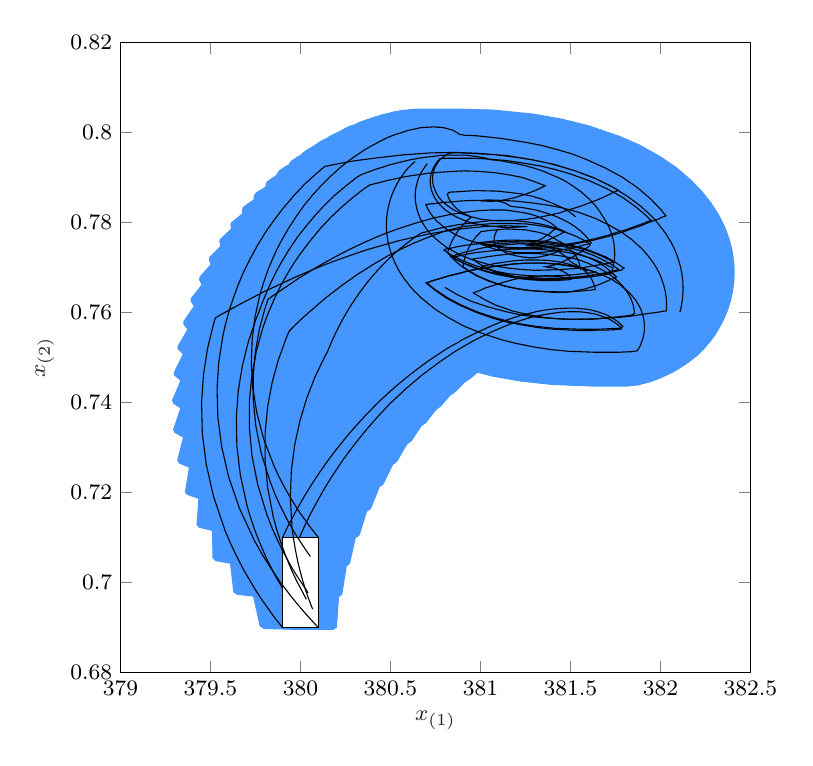
\begin{tikzpicture}
\footnotesize

\begin{axis}[%
width=8cm,
height=8cm,
at={(0in,0in)},
scale only axis,
xmin=379,
xmax=382.5,
xlabel style={font=\color{white!15!black}},
xlabel={$x_{(1)}$},
ymin=0.68,
ymax=0.82,
ylabel style={font=\color{white!15!black}},
ylabel={$x_{(2)}$},
axis background/.style={fill=white}
]

\addplot[area legend, draw=mycolor1, fill=mycolor1, forget plot]
table[row sep=crcr] {%
x	y\\
380.1809	0.6896\\
379.9887	0.6896\\
379.7979	0.6898\\
379.776	0.6904\\
379.7396	0.697\\
379.6488	0.6974\\
379.6301	0.6979\\
379.6115	0.7043\\
379.53	0.7049\\
379.5142	0.7055\\
379.5114	0.7116\\
379.4385	0.7123\\
379.4254	0.7129\\
379.4361	0.7187\\
379.3718	0.7196\\
379.3611	0.7201\\
379.3833	0.7256\\
379.3271	0.7266\\
379.3187	0.7272\\
379.3506	0.7323\\
379.3021	0.7334\\
379.2957	0.734\\
379.3357	0.7388\\
379.2942	0.7399\\
379.2896	0.7405\\
379.3362	0.7449\\
379.3014	0.7461\\
379.2984	0.7466\\
379.3501	0.7508\\
379.3214	0.7519\\
379.3199	0.7525\\
379.3755	0.7563\\
379.3524	0.7574\\
379.3521	0.758\\
379.4106	0.7614\\
379.3925	0.7626\\
379.3934	0.7631\\
379.4538	0.7662\\
379.4402	0.7673\\
379.442	0.7679\\
379.5036	0.7707\\
379.4939	0.7718\\
379.4967	0.7723\\
379.5586	0.7748\\
379.5523	0.7758\\
379.5559	0.7763\\
379.6175	0.7786\\
379.6142	0.7795\\
379.6186	0.78\\
379.6794	0.782\\
379.6784	0.7829\\
379.6836	0.7834\\
379.6959	0.7838\\
379.7429	0.7851\\
379.744	0.786\\
379.7508	0.7864\\
379.7618	0.7868\\
379.7793	0.7872\\
379.8076	0.7879\\
379.8101	0.7887\\
379.8171	0.7891\\
379.8282	0.7894\\
379.8457	0.7899\\
379.863	0.7903\\
379.876	0.7911\\
379.8836	0.7915\\
379.8942	0.7918\\
379.9118	0.7923\\
379.9291	0.7927\\
379.9457	0.793\\
380.0016	0.7941\\
380.0171	0.7944\\
380.032	0.7946\\
380.0461	0.7948\\
380.1976	0.7967\\
380.2108	0.7968\\
380.2231	0.7969\\
380.2396	0.797\\
380.4451	0.797\\
380.6253	0.7968\\
380.7967	0.7961\\
380.9507	0.795\\
381.0881	0.7936\\
381.2096	0.792\\
381.3162	0.7901\\
381.4088	0.7881\\
381.4884	0.7859\\
381.5558	0.7836\\
381.6107	0.7814\\
381.6543	0.7792\\
381.689	0.777\\
381.7156	0.7748\\
381.735	0.7727\\
381.7479	0.7706\\
381.7551	0.7686\\
381.7573	0.7667\\
381.7551	0.7648\\
381.7491	0.7631\\
381.7394	0.7614\\
381.7318	0.7609\\
381.7212	0.7606\\
381.7036	0.7602\\
381.6863	0.7597\\
381.6697	0.7594\\
381.6138	0.7583\\
381.5983	0.7581\\
381.5833	0.7578\\
381.5692	0.7576\\
381.4178	0.7558\\
381.4046	0.7556\\
381.3923	0.7555\\
381.372	0.7553\\
381.3579	0.7551\\
381.3447	0.7549\\
381.3231	0.7546\\
381.3081	0.7544\\
381.294	0.7542\\
381.2712	0.7537\\
381.2554	0.7535\\
381.2404	0.7532\\
381.2165	0.7527\\
381.1999	0.7524\\
381.1841	0.7521\\
381.1592	0.7515\\
381.1418	0.7511\\
381.1252	0.7507\\
381.1083	0.7503\\
381.0903	0.7498\\
381.0726	0.7494\\
381.0585	0.749\\
381.0286	0.7481\\
381.0101	0.7476\\
380.9924	0.7471\\
380.9468	0.7455\\
380.9279	0.745\\
380.913	0.7446\\
380.8637	0.7426\\
380.8447	0.742\\
380.8339	0.7418\\
380.7801	0.7393\\
380.7698	0.739\\
380.7529	0.7385\\
380.6968	0.7356\\
380.6865	0.7353\\
380.6716	0.7349\\
380.6149	0.7315\\
380.6046	0.7312\\
380.591	0.7308\\
380.5355	0.727\\
380.5253	0.7266\\
380.5124	0.7263\\
380.4601	0.722\\
380.4499	0.7216\\
380.4375	0.7213\\
380.39	0.7165\\
380.38	0.7162\\
380.3676	0.7159\\
380.327	0.7107\\
380.3171	0.7103\\
380.3047	0.71\\
380.2727	0.7043\\
380.2543	0.7037\\
380.2296	0.6974\\
380.2115	0.6969\\
380.1996	0.6901\\
380.1813	0.6896\\
}--cycle;

\addplot[area legend, draw=mycolor1, fill=mycolor1, forget plot]
table[row sep=crcr] {%
x	y\\
380.583	0.7593\\
380.4615	0.761\\
380.3548	0.7629\\
380.2622	0.7649\\
380.1827	0.7671\\
380.1153	0.7693\\
380.059	0.7716\\
380.0141	0.7739\\
379.9795	0.7761\\
379.9528	0.7783\\
379.9334	0.7804\\
379.9205	0.7825\\
379.9133	0.7844\\
379.9111	0.7864\\
379.9133	0.7882\\
379.9193	0.79\\
379.9285	0.7916\\
379.9411	0.7932\\
379.9487	0.7936\\
379.9594	0.7939\\
379.9681	0.7941\\
379.9769	0.7944\\
379.9858	0.7946\\
379.9946	0.7948\\
380.0043	0.795\\
380.0128	0.7954\\
380.023	0.7957\\
380.0318	0.796\\
380.0494	0.7964\\
380.0583	0.7966\\
380.0708	0.7969\\
380.0847	0.7973\\
380.0935	0.7975\\
380.1023	0.7978\\
380.1112	0.798\\
380.12	0.7982\\
380.1362	0.7985\\
380.1477	0.7987\\
380.1617	0.7991\\
380.1795	0.7995\\
380.1957	0.7998\\
380.2115	0.8001\\
380.2224	0.8003\\
380.2359	0.8006\\
380.2525	0.801\\
380.2684	0.8013\\
380.2984	0.8017\\
380.3147	0.802\\
380.3301	0.8023\\
380.3446	0.8025\\
380.3582	0.8027\\
380.3734	0.8029\\
380.3884	0.8031\\
380.4025	0.8033\\
380.4157	0.8035\\
380.429	0.8036\\
380.4435	0.8038\\
380.4572	0.804\\
380.4699	0.8041\\
380.4817	0.8042\\
380.4951	0.8043\\
380.5083	0.8045\\
380.5206	0.8046\\
380.5373	0.8047\\
380.5498	0.8048\\
380.5621	0.8049\\
380.5788	0.805\\
380.5944	0.805\\
380.6062	0.8051\\
380.6222	0.8051\\
380.6402	0.8052\\
380.8897	0.8052\\
381.07	0.805\\
381.0959	0.8049\\
381.2707	0.8042\\
381.294	0.8041\\
381.451	0.803\\
381.4718	0.8028\\
381.6118	0.8014\\
381.6303	0.8011\\
381.7542	0.7994\\
381.7705	0.7992\\
381.8792	0.7973\\
381.8933	0.797\\
381.9878	0.7949\\
381.9999	0.7946\\
382.0811	0.7924\\
382.1486	0.7901\\
382.2049	0.7878\\
382.2509	0.7855\\
382.2876	0.7832\\
382.2939	0.7827\\
382.3205	0.7805\\
382.3411	0.7783\\
382.3549	0.7761\\
382.3606	0.7749\\
382.3679	0.7729\\
382.3703	0.7709\\
382.3681	0.7689\\
382.362	0.7671\\
382.3524	0.7654\\
382.34	0.7638\\
382.3251	0.7623\\
382.3083	0.761\\
382.2899	0.7597\\
382.2705	0.7585\\
382.2504	0.7575\\
382.2298	0.7565\\
382.209	0.7557\\
382.1883	0.7549\\
382.1683	0.7542\\
382.1492	0.7537\\
382.1399	0.7534\\
382.1223	0.753\\
382.1042	0.7525\\
382.0954	0.7523\\
382.0695	0.7517\\
382.0528	0.7513\\
382.0361	0.751\\
382.0203	0.7507\\
382.0044	0.7505\\
381.9894	0.7502\\
381.9744	0.75\\
381.9462	0.7496\\
381.933	0.7495\\
381.9196	0.7494\\
381.9076	0.7493\\
381.8951	0.7492\\
381.8718	0.7491\\
381.8568	0.749\\
381.6614	0.749\\
381.481	0.7493\\
381.3094	0.7499\\
381.1552	0.751\\
381.0177	0.7524\\
380.8945	0.7541\\
380.7878	0.756\\
380.695	0.758\\
380.6855	0.7583\\
380.583	0.7593\\
}--cycle;

\addplot[area legend, draw=mycolor1, fill=mycolor1, forget plot]
table[row sep=crcr] {%
x	y\\
380.4071	0.7924\\
380.4265	0.7936\\
380.4467	0.7947\\
380.4673	0.7956\\
380.4881	0.7965\\
380.5088	0.7972\\
380.5292	0.7979\\
380.5488	0.7985\\
380.5581	0.7987\\
380.5669	0.799\\
380.5756	0.7992\\
380.5938	0.7997\\
380.6026	0.7999\\
380.6111	0.8001\\
380.6285	0.8005\\
380.6452	0.8008\\
380.6618	0.8011\\
380.6936	0.8017\\
380.7085	0.8019\\
380.7235	0.8022\\
380.7377	0.8023\\
380.7518	0.8025\\
380.765	0.8027\\
380.7781	0.8028\\
380.7904	0.8029\\
380.8026	0.803\\
380.814	0.803\\
380.8255	0.8031\\
380.8469	0.8031\\
381.047	0.8032\\
381.2273	0.8029\\
381.3989	0.8022\\
381.553	0.8012\\
381.6905	0.7998\\
381.8122	0.7981\\
381.9203	0.7962\\
382.013	0.7942\\
382.0927	0.792\\
382.1602	0.7897\\
382.1689	0.7894\\
382.2262	0.7871\\
382.2334	0.7867\\
382.2803	0.7844\\
382.286	0.784\\
382.3235	0.7817\\
382.3279	0.7813\\
382.3567	0.779\\
382.3599	0.7787\\
382.381	0.7764\\
382.3832	0.7761\\
382.3973	0.7739\\
382.3986	0.7735\\
382.4066	0.7714\\
382.4071	0.7711\\
382.4097	0.7691\\
382.4095	0.7688\\
382.4073	0.7668\\
382.4065	0.7665\\
382.4003	0.7647\\
382.3987	0.7644\\
382.3894	0.7627\\
382.3872	0.7624\\
382.375	0.7608\\
382.3721	0.7605\\
382.3578	0.7591\\
382.3544	0.7588\\
382.3383	0.7575\\
382.3342	0.7572\\
382.3127	0.7557\\
382.2945	0.7546\\
382.2711	0.7534\\
382.2472	0.7523\\
382.223	0.7513\\
382.2023	0.7505\\
382.1819	0.7499\\
382.1618	0.7493\\
382.1525	0.749\\
382.1429	0.7488\\
382.1341	0.7485\\
382.116	0.7481\\
382.1062	0.7478\\
382.0978	0.7476\\
382.0773	0.7472\\
382.068	0.747\\
382.0432	0.7465\\
382.0265	0.7462\\
382.0107	0.7459\\
382.0012	0.7457\\
381.9866	0.7455\\
381.9716	0.7453\\
381.9568	0.7451\\
381.9427	0.7449\\
381.9288	0.7448\\
381.9157	0.7447\\
381.9028	0.7445\\
381.8906	0.7445\\
381.8787	0.7444\\
381.8671	0.7443\\
381.6449	0.7443\\
381.4548	0.7445\\
381.4377	0.7445\\
381.2743	0.7452\\
381.2588	0.7453\\
381.1121	0.7463\\
381.0982	0.7465\\
380.9673	0.7478\\
380.955	0.7479\\
380.8393	0.7495\\
380.8284	0.7497\\
380.7269	0.7515\\
380.7174	0.7517\\
380.6292	0.7537\\
380.621	0.7539\\
380.5454	0.7559\\
380.4745	0.7583\\
380.4153	0.7607\\
380.3668	0.7631\\
380.3282	0.7656\\
380.2985	0.768\\
380.2768	0.7703\\
380.2622	0.7726\\
380.254	0.7748\\
380.2514	0.7769\\
380.2536	0.7789\\
380.26	0.7808\\
380.2695	0.7825\\
380.2819	0.7841\\
380.2969	0.7856\\
380.3137	0.787\\
380.3321	0.7883\\
380.3517	0.7895\\
380.3719	0.7905\\
380.3925	0.7915\\
380.4071	0.7924\\
}--cycle;

\addplot[area legend, draw=mycolor1, fill=mycolor1, forget plot]
table[row sep=crcr] {%
x	y\\
381.6659	0.7958\\
381.6782	0.7957\\
381.794	0.7941\\
381.8049	0.7939\\
381.9064	0.7921\\
381.9159	0.7919\\
382.004	0.7899\\
382.0122	0.7897\\
382.0879	0.7877\\
382.095	0.7875\\
382.1589	0.7853\\
382.2182	0.7829\\
382.2666	0.7805\\
382.3052	0.778\\
382.3349	0.7756\\
382.3566	0.7733\\
382.3712	0.771\\
382.3794	0.7688\\
382.3821	0.7667\\
382.3799	0.7646\\
382.3735	0.7628\\
382.3635	0.761\\
382.3511	0.7594\\
382.3361	0.7579\\
382.3193	0.7565\\
382.301	0.7552\\
382.2815	0.754\\
382.2611	0.753\\
382.2405	0.752\\
382.2197	0.7512\\
382.199	0.7504\\
382.1752	0.7496\\
382.1519	0.7489\\
382.1426	0.7487\\
382.1298	0.7483\\
382.121	0.7481\\
382.1029	0.7476\\
382.0901	0.7473\\
382.0817	0.7471\\
382.0642	0.7467\\
382.052	0.7465\\
382.0271	0.746\\
382.0155	0.7458\\
381.9919	0.7454\\
381.9808	0.7452\\
381.9585	0.7449\\
381.9481	0.7447\\
381.9271	0.7445\\
381.911	0.7443\\
381.8978	0.7442\\
381.8828	0.744\\
381.8705	0.7439\\
381.8566	0.7439\\
381.8451	0.7438\\
381.8326	0.7438\\
381.8215	0.7437\\
381.6192	0.7437\\
381.4291	0.744\\
381.4104	0.744\\
381.247	0.7447\\
381.2302	0.7448\\
381.0834	0.7458\\
381.0683	0.7459\\
380.9375	0.7473\\
380.9241	0.7474\\
380.8083	0.749\\
380.7965	0.7492\\
380.6949	0.751\\
380.6846	0.7512\\
380.5964	0.7532\\
380.5882	0.7534\\
380.5054	0.7557\\
380.4414	0.7578\\
380.3821	0.7602\\
380.3336	0.7627\\
380.2945	0.7651\\
380.2647	0.7675\\
380.243	0.7699\\
380.2408	0.7702\\
380.2279	0.7722\\
380.2197	0.7744\\
380.217	0.7765\\
380.2192	0.7786\\
380.2256	0.7805\\
380.2356	0.7823\\
380.2486	0.784\\
380.2642	0.7855\\
380.2819	0.787\\
380.3011	0.7883\\
380.3215	0.7896\\
380.3426	0.7907\\
380.3642	0.7917\\
380.386	0.7926\\
380.4077	0.7934\\
380.4291	0.7941\\
380.4501	0.7947\\
380.4594	0.7949\\
380.47	0.7952\\
380.4788	0.7955\\
380.4969	0.7959\\
380.5075	0.7962\\
380.516	0.7964\\
380.5334	0.7968\\
380.5436	0.797\\
380.5684	0.7975\\
380.5781	0.7977\\
380.6017	0.7981\\
380.6182	0.7983\\
380.6332	0.7986\\
380.6488	0.7988\\
380.6628	0.7989\\
380.6774	0.7991\\
380.6905	0.7992\\
380.7041	0.7993\\
380.7163	0.7994\\
380.7282	0.7995\\
380.7398	0.7995\\
380.7609	0.7996\\
380.9623	0.7996\\
381.1524	0.7994\\
381.1695	0.7993\\
381.3329	0.7987\\
381.3484	0.7986\\
381.4951	0.7975\\
381.5091	0.7974\\
381.6399	0.7961\\
381.6498	0.796\\
381.6659	0.7958\\
}--cycle;

\addplot[area legend, draw=mycolor1, fill=mycolor1, forget plot]
table[row sep=crcr] {%
x	y\\
381.6114	0.7438\\
381.4213	0.7441\\
381.4042	0.7441\\
381.2408	0.7448\\
381.2254	0.7448\\
381.0786	0.7459\\
381.0647	0.746\\
380.9339	0.7473\\
380.9215	0.7475\\
380.8057	0.7491\\
380.7949	0.7493\\
380.6934	0.7511\\
380.6839	0.7512\\
380.5957	0.7532\\
380.5875	0.7534\\
380.5118	0.7555\\
380.5042	0.7557\\
380.4401	0.7579\\
380.4337	0.7581\\
380.3802	0.7603\\
380.3748	0.7605\\
380.3312	0.7627\\
380.2922	0.7652\\
380.2621	0.7676\\
380.2401	0.77\\
380.2254	0.7723\\
380.2171	0.7745\\
380.2144	0.7766\\
380.2143	0.7769\\
380.2166	0.7787\\
380.223	0.7807\\
380.233	0.7825\\
380.2461	0.7841\\
380.2619	0.7857\\
380.2796	0.7872\\
380.299	0.7886\\
380.3195	0.7898\\
380.3408	0.7909\\
380.3626	0.7919\\
380.3844	0.7928\\
380.4062	0.7936\\
380.4276	0.7943\\
380.4486	0.7949\\
380.4579	0.7952\\
380.4687	0.7955\\
380.4774	0.7957\\
380.4956	0.7962\\
380.5062	0.7964\\
380.5147	0.7966\\
380.5321	0.797\\
380.5423	0.7972\\
380.5672	0.7977\\
380.5773	0.7979\\
380.601	0.7983\\
380.6175	0.7986\\
380.6325	0.7988\\
380.648	0.799\\
380.6621	0.7992\\
380.6766	0.7993\\
380.6898	0.7995\\
380.7033	0.7996\\
380.7158	0.7997\\
380.728	0.7997\\
380.7395	0.7998\\
380.7508	0.7998\\
380.7616	0.7999\\
380.9642	0.7999\\
381.1538	0.7996\\
381.1713	0.7996\\
381.3346	0.7989\\
381.3505	0.7988\\
381.4973	0.7978\\
381.5115	0.7977\\
381.6423	0.7963\\
381.655	0.7962\\
381.7708	0.7946\\
381.7819	0.7944\\
381.8834	0.7926\\
381.8931	0.7924\\
381.9813	0.7905\\
381.9897	0.7903\\
382.0654	0.7882\\
382.0726	0.788\\
382.1367	0.7858\\
382.1962	0.7834\\
382.2448	0.781\\
382.2837	0.7785\\
382.3135	0.7761\\
382.3353	0.7738\\
382.35	0.7715\\
382.3582	0.7693\\
382.3609	0.7672\\
382.3609	0.7669\\
382.3587	0.765\\
382.3523	0.7632\\
382.3423	0.7614\\
382.3293	0.7597\\
382.3137	0.7581\\
382.296	0.7567\\
382.2768	0.7553\\
382.2725	0.755\\
382.2529	0.7539\\
382.2317	0.7527\\
382.2101	0.7517\\
382.1883	0.7508\\
382.1666	0.7501\\
382.1452	0.7494\\
382.1242	0.7487\\
382.1149	0.7485\\
382.1043	0.7482\\
382.0955	0.748\\
382.0774	0.7475\\
382.0668	0.7472\\
382.0583	0.747\\
382.0409	0.7466\\
382.0307	0.7464\\
382.0059	0.7459\\
381.9962	0.7458\\
381.9726	0.7453\\
381.9561	0.7451\\
381.9411	0.7449\\
381.9256	0.7447\\
381.9115	0.7445\\
381.8969	0.7443\\
381.8838	0.7442\\
381.8703	0.7441\\
381.858	0.744\\
381.8455	0.7439\\
381.834	0.7439\\
381.8233	0.7438\\
381.6114	0.7438\\
}--cycle;

\addplot[area legend, draw=black, fill=white, forget plot]
table[row sep=crcr] {%
x	y\\
379.9	0.69\\
380.1	0.69\\
380.1	0.71\\
379.9	0.71\\
379.9	0.69\\
}--cycle;
\addplot [color=black, forget plot]
  table[row sep=crcr]{%
379.9	0.69\\
379.8905	0.6905\\
379.8811	0.691\\
379.8659	0.6917\\
379.8228	0.6941\\
379.7892	0.696\\
379.7574	0.6979\\
379.7274	0.6999\\
379.6847	0.7028\\
379.6461	0.7058\\
379.6115	0.7087\\
379.5808	0.7116\\
379.5174	0.7191\\
379.4763	0.7263\\
379.4548	0.7332\\
379.4506	0.7399\\
379.4612	0.7462\\
379.4848	0.7522\\
379.5191	0.7578\\
379.527	0.7588\\
379.5504	0.7594\\
379.5737	0.7599\\
379.5968	0.7604\\
379.6653	0.7619\\
379.7328	0.7633\\
379.7995	0.7647\\
379.8652	0.7659\\
379.9721	0.7679\\
380.0762	0.7697\\
380.1774	0.7713\\
380.2757	0.7727\\
380.371	0.774\\
380.5486	0.776\\
380.7143	0.7775\\
380.868	0.7785\\
381.0098	0.7791\\
381.1398	0.7793\\
381.2604	0.7791\\
381.2418	0.7791\\
381.201	0.779\\
381.1705	0.7789\\
381.1413	0.7789\\
381.1132	0.779\\
381.0551	0.7792\\
381.0028	0.7795\\
380.9642	0.7798\\
380.9291	0.7802\\
380.8975	0.7807\\
380.8691	0.7812\\
380.8386	0.7819\\
380.8124	0.7826\\
380.7997	0.783\\
380.7893	0.7834\\
380.7745	0.784\\
380.7618	0.7846\\
380.7512	0.7852\\
380.7424	0.7858\\
380.7337	0.7866\\
380.7275	0.7873\\
380.7235	0.788\\
380.7215	0.7887\\
380.7211	0.7894\\
380.7222	0.79\\
380.7244	0.7905\\
380.7287	0.7912\\
380.7375	0.7921\\
380.7488	0.7929\\
380.7617	0.7936\\
380.7751	0.7942\\
380.7919	0.7943\\
380.9676	0.7943\\
381.0141	0.7942\\
381.1448	0.7938\\
381.2414	0.7932\\
381.3316	0.7926\\
381.4156	0.7918\\
381.4935	0.7909\\
381.6061	0.7893\\
381.7047	0.7875\\
381.7902	0.7856\\
381.8635	0.7835\\
381.9255	0.7814\\
381.9483	0.7805\\
381.9331	0.7803\\
381.918	0.78\\
381.903	0.7798\\
381.8551	0.7791\\
381.8082	0.7784\\
381.7624	0.7779\\
381.7177	0.7773\\
381.6338	0.7764\\
381.554	0.7757\\
381.4783	0.7752\\
381.4067	0.7748\\
381.3122	0.7745\\
381.2257	0.7744\\
381.1471	0.7745\\
381.0894	0.7748\\
381.0365	0.7751\\
380.9894	0.7756\\
381.0019	0.7756\\
381.0266	0.7757\\
381.069	0.7759\\
381.1103	0.776\\
381.1503	0.7761\\
381.1892	0.7761\\
381.2976	0.776\\
381.375	0.7758\\
381.4463	0.7754\\
381.5118	0.7749\\
381.5717	0.7743\\
381.6404	0.7733\\
381.7008	0.7723\\
381.7532	0.7711\\
381.7982	0.7699\\
381.7802	0.7694\\
381.7663	0.7693\\
381.7194	0.7689\\
381.6737	0.7686\\
381.6292	0.7684\\
381.5858	0.7681\\
381.4645	0.7677\\
381.3531	0.7676\\
381.2687	0.7678\\
381.1907	0.768\\
381.119	0.7685\\
381.0534	0.769\\
380.979	0.7699\\
380.9135	0.7709\\
380.8562	0.772\\
380.8404	0.7723\\
380.8539	0.7724\\
380.8673	0.7725\\
380.8806	0.7726\\
380.9256	0.773\\
380.9694	0.7733\\
381.0121	0.7735\\
381.0537	0.7737\\
381.1694	0.7741\\
381.2751	0.7742\\
381.3537	0.774\\
381.4261	0.7737\\
381.4925	0.7733\\
381.5532	0.7728\\
381.6204	0.772\\
381.6796	0.771\\
381.7312	0.77\\
};
\addplot [color=black, forget plot]
  table[row sep=crcr]{%
380.1	0.69\\
380.0808	0.6908\\
380.0714	0.6912\\
380.0373	0.6927\\
380.0045	0.6942\\
379.9731	0.6957\\
379.9429	0.6972\\
379.8859	0.7002\\
379.8339	0.7033\\
379.7869	0.7063\\
379.7446	0.7093\\
379.661	0.7165\\
379.6009	0.7235\\
379.5617	0.7303\\
379.541	0.7368\\
379.5366	0.7431\\
379.5462	0.749\\
379.568	0.7546\\
379.578	0.7565\\
379.5815	0.7571\\
379.585	0.7576\\
379.5887	0.7582\\
379.6083	0.761\\
379.6303	0.7636\\
379.6544	0.7662\\
379.6805	0.7687\\
379.7199	0.7719\\
379.762	0.775\\
379.8064	0.7779\\
379.8525	0.7805\\
379.8999	0.783\\
379.9633	0.786\\
380.0274	0.7887\\
380.0913	0.791\\
380.1352	0.7925\\
380.1533	0.7926\\
380.1713	0.7928\\
380.1893	0.7929\\
380.2503	0.7934\\
380.3103	0.7938\\
380.369	0.7941\\
380.4266	0.7944\\
380.5812	0.7951\\
380.7267	0.7955\\
380.8634	0.7956\\
380.9914	0.7954\\
381.1461	0.7949\\
381.2867	0.794\\
381.4136	0.7929\\
381.5275	0.7915\\
381.629	0.79\\
381.7268	0.7881\\
381.7658	0.7872\\
381.7517	0.7869\\
381.7376	0.7867\\
381.7236	0.7864\\
381.6815	0.7856\\
381.6402	0.7849\\
381.5999	0.7843\\
381.5606	0.7837\\
381.4958	0.7829\\
381.434	0.7821\\
381.3752	0.7816\\
381.3194	0.7811\\
381.2469	0.7807\\
381.1801	0.7805\\
381.1191	0.7804\\
381.0636	0.7805\\
381.0126	0.7807\\
380.9994	0.7808\\
380.9692	0.7811\\
380.9469	0.7813\\
380.9259	0.7816\\
380.9063	0.7818\\
380.8776	0.7823\\
380.8522	0.7828\\
380.8298	0.7834\\
380.8103	0.784\\
380.7912	0.7846\\
380.7754	0.7853\\
380.7626	0.786\\
380.7533	0.7867\\
380.7418	0.7878\\
380.7374	0.7884\\
380.7349	0.789\\
380.7339	0.7896\\
380.7344	0.7902\\
380.7361	0.7908\\
380.7425	0.7918\\
380.7486	0.7924\\
380.7562	0.7929\\
380.7673	0.7936\\
380.7791	0.7941\\
380.7912	0.7945\\
380.8029	0.7949\\
380.8168	0.7952\\
380.8307	0.7954\\
380.8453	0.7955\\
380.8907	0.7955\\
380.9398	0.7954\\
380.9876	0.7953\\
381.0342	0.7952\\
381.0796	0.7951\\
381.2025	0.7945\\
381.294	0.7939\\
381.3796	0.7932\\
381.4593	0.7923\\
381.5333	0.7914\\
381.6432	0.7897\\
381.739	0.7878\\
381.8218	0.7857\\
381.8924	0.7836\\
381.9518	0.7814\\
381.9787	0.7802\\
381.9886	0.7797\\
382.012	0.7785\\
382.029	0.7776\\
382.0443	0.7766\\
382.0582	0.7757\\
382.0759	0.7743\\
382.0905	0.7729\\
382.1024	0.7715\\
382.1116	0.7702\\
382.1184	0.7689\\
382.1247	0.7669\\
382.126	0.765\\
382.123	0.7632\\
382.1163	0.7614\\
382.1083	0.7601\\
};
\addplot [color=black, forget plot]
  table[row sep=crcr]{%
380.1	0.71\\
380.0905	0.7105\\
380.0626	0.7119\\
380.0404	0.7131\\
380.019	0.7143\\
379.9986	0.7154\\
379.9561	0.7181\\
379.9178	0.7207\\
379.8835	0.7233\\
379.8532	0.7259\\
379.7958	0.7319\\
379.7571	0.7378\\
379.7348	0.7435\\
379.7269	0.7489\\
379.7317	0.7541\\
379.7474	0.759\\
379.7722	0.7636\\
379.7857	0.7655\\
379.79	0.766\\
379.7943	0.7666\\
379.7988	0.7671\\
379.8198	0.7695\\
379.8426	0.7717\\
379.8672	0.7739\\
379.8932	0.7759\\
379.9333	0.7787\\
379.9756	0.7813\\
380.0195	0.7838\\
380.0644	0.786\\
380.1099	0.788\\
380.1648	0.7902\\
380.2194	0.7922\\
380.2732	0.7939\\
380.2948	0.7945\\
380.3078	0.7949\\
380.3207	0.7952\\
380.3499	0.796\\
380.3786	0.7967\\
380.4066	0.7973\\
380.434	0.7979\\
380.4785	0.7988\\
380.5209	0.7995\\
380.561	0.8\\
380.5987	0.8005\\
380.634	0.8008\\
380.6683	0.8011\\
380.6999	0.8012\\
380.7115	0.8012\\
380.7427	0.8013\\
380.7613	0.8012\\
380.7787	0.8012\\
380.7947	0.8011\\
380.8146	0.8009\\
380.8324	0.8007\\
380.848	0.8005\\
380.8617	0.8002\\
380.8735	0.7999\\
380.8836	0.7996\\
380.902	0.7995\\
380.9161	0.7994\\
380.93	0.7994\\
380.9791	0.7993\\
381.0269	0.7991\\
381.0735	0.7989\\
381.1189	0.7987\\
381.2573	0.7978\\
381.3463	0.7971\\
381.4295	0.7962\\
381.507	0.7953\\
381.5791	0.7942\\
381.6909	0.7922\\
381.7879	0.7901\\
381.8712	0.7878\\
381.9417	0.7854\\
382.0006	0.783\\
382.0303	0.7815\\
382.0144	0.7813\\
381.9986	0.781\\
381.9829	0.7807\\
381.9335	0.78\\
381.885	0.7792\\
381.8376	0.7786\\
381.7912	0.7779\\
381.708	0.7769\\
381.6284	0.7761\\
381.5526	0.7755\\
381.4805	0.7749\\
381.3795	0.7744\\
381.2868	0.7742\\
381.2021	0.7742\\
381.1253	0.7744\\
381.056	0.7748\\
381.0211	0.7751\\
381.0065	0.7752\\
380.973	0.7756\\
380.948	0.7759\\
380.9245	0.7762\\
380.9023	0.7766\\
380.868	0.7772\\
380.8372	0.7779\\
380.8098	0.7786\\
380.7856	0.7794\\
380.7588	0.7803\\
380.7366	0.7813\\
380.7187	0.7823\\
380.7046	0.7833\\
380.6968	0.784\\
380.7262	0.7842\\
380.7407	0.7842\\
380.7906	0.7845\\
380.8394	0.7846\\
380.887	0.7848\\
380.9334	0.7849\\
381.0847	0.785\\
381.1877	0.7848\\
381.2833	0.7844\\
381.3717	0.7839\\
381.4532	0.7833\\
381.5527	0.7822\\
381.6405	0.7809\\
381.7173	0.7794\\
381.7838	0.7779\\
381.8211	0.7768\\
381.8328	0.7765\\
381.8604	0.7755\\
381.8807	0.7748\\
381.8995	0.7741\\
381.9168	0.7733\\
381.9398	0.7722\\
381.9599	0.7711\\
381.9772	0.77\\
381.9918	0.7689\\
382.004	0.7678\\
382.0185	0.7661\\
382.028	0.7645\\
382.0331	0.763\\
382.0343	0.7615\\
382.0329	0.7604\\
382.0017	0.7602\\
381.9862	0.7601\\
381.9334	0.7598\\
381.8818	0.7595\\
381.8313	0.7592\\
381.7821	0.759\\
381.6369	0.7586\\
381.5029	0.7585\\
381.4026	0.7587\\
381.3092	0.759\\
381.2225	0.7595\\
381.1424	0.7602\\
381.0404	0.7613\\
380.9503	0.7625\\
380.8713	0.764\\
380.8024	0.7656\\
};
\addplot [color=black, forget plot]
  table[row sep=crcr]{%
379.9	0.71\\
379.9096	0.7108\\
379.9193	0.7116\\
379.9291	0.7124\\
379.9739	0.7158\\
380.0204	0.7191\\
380.0605	0.7217\\
380.1015	0.7242\\
380.1434	0.7266\\
380.1859	0.7289\\
380.27	0.7331\\
380.3554	0.7369\\
380.4411	0.7404\\
380.5266	0.7435\\
380.6112	0.7463\\
380.7079	0.7492\\
380.8018	0.7517\\
380.8487	0.7528\\
380.8631	0.7531\\
380.8774	0.7534\\
380.8917	0.7538\\
380.9316	0.7546\\
380.9707	0.7554\\
381.0091	0.7561\\
381.0465	0.7568\\
381.1062	0.7578\\
381.1635	0.7586\\
381.218	0.7593\\
381.27	0.7598\\
381.3192	0.7603\\
381.3807	0.7607\\
381.4375	0.7609\\
381.4895	0.761\\
381.5351	0.761\\
381.5485	0.7609\\
381.579	0.7608\\
381.6015	0.7607\\
381.6226	0.7605\\
381.6424	0.7603\\
381.6732	0.7599\\
381.7004	0.7595\\
381.7243	0.759\\
381.745	0.7585\\
381.7633	0.758\\
381.7786	0.7574\\
381.7913	0.7569\\
381.7812	0.7566\\
381.767	0.7565\\
381.7529	0.7565\\
381.704	0.7564\\
381.6563	0.7563\\
381.5646	0.7563\\
381.4149	0.7565\\
381.321	0.7569\\
381.2337	0.7574\\
381.1528	0.7581\\
381.078	0.7589\\
380.9791	0.7602\\
380.8923	0.7617\\
380.8169	0.7633\\
380.752	0.765\\
380.7025	0.7666\\
380.7315	0.767\\
380.7458	0.7672\\
380.7927	0.7678\\
380.8385	0.7683\\
380.8832	0.7687\\
380.9269	0.7692\\
381.0181	0.7699\\
381.104	0.7704\\
381.1847	0.7708\\
381.2602	0.771\\
381.3507	0.771\\
381.4327	0.7707\\
381.5067	0.7703\\
381.5729	0.7698\\
381.6317	0.7691\\
381.6419	0.7689\\
381.6549	0.7687\\
381.6851	0.7682\\
381.7076	0.7678\\
381.7285	0.7674\\
381.7481	0.7669\\
381.7752	0.7662\\
381.7993	0.7654\\
381.8205	0.7647\\
381.8391	0.7639\\
381.8604	0.7629\\
381.8773	0.7618\\
381.8904	0.7608\\
381.9	0.7597\\
381.9053	0.759\\
381.908	0.7584\\
381.9108	0.7574\\
381.9113	0.7565\\
381.9102	0.7559\\
381.9079	0.7552\\
381.9046	0.7546\\
381.9004	0.754\\
381.8942	0.7533\\
381.8871	0.7526\\
381.8791	0.752\\
381.8707	0.7515\\
381.8542	0.7514\\
381.8393	0.7513\\
381.8246	0.7513\\
381.7735	0.7512\\
381.6273	0.7512\\
381.489	0.7514\\
381.3874	0.7518\\
381.2926	0.7524\\
381.2044	0.7531\\
381.1225	0.7539\\
381.0086	0.7554\\
380.9086	0.757\\
380.8215	0.7589\\
380.7464	0.7608\\
380.6827	0.7629\\
380.667	0.7634\\
380.6558	0.7639\\
380.6296	0.7649\\
380.6105	0.7658\\
380.5928	0.7667\\
380.5767	0.7675\\
380.5554	0.7688\\
380.537	0.7701\\
380.5215	0.7714\\
380.5087	0.7726\\
380.4982	0.7739\\
380.4861	0.7758\\
380.4793	0.7777\\
380.4774	0.7796\\
380.4796	0.7813\\
380.4853	0.7829\\
380.4885	0.7835\\
380.4982	0.785\\
380.5075	0.7861\\
380.5181	0.7871\\
380.5298	0.7881\\
380.5459	0.7893\\
380.563	0.7903\\
380.5809	0.7913\\
380.5992	0.7922\\
380.6362	0.7936\\
};
\addplot [color=black, forget plot]
  table[row sep=crcr]{%
379.9946	0.71\\
380.0029	0.7108\\
380.0114	0.7115\\
380.02	0.7123\\
380.0562	0.7153\\
380.0939	0.7181\\
380.1331	0.7209\\
380.1735	0.7235\\
380.2349	0.7272\\
380.298	0.7306\\
380.3624	0.7338\\
380.4276	0.7368\\
380.4932	0.7396\\
380.5861	0.7431\\
380.678	0.7462\\
380.7683	0.7489\\
380.8561	0.7513\\
380.8728	0.7517\\
380.8873	0.752\\
380.9017	0.7524\\
380.916	0.7527\\
380.9548	0.7536\\
380.9929	0.7544\\
381.0302	0.7551\\
381.0667	0.7558\\
381.1253	0.7568\\
381.1814	0.7577\\
381.2349	0.7584\\
381.2857	0.759\\
381.3339	0.7594\\
381.3922	0.7598\\
381.446	0.7601\\
381.4953	0.7602\\
381.5432	0.7602\\
381.5734	0.7601\\
381.5957	0.76\\
381.6167	0.7598\\
381.6363	0.7597\\
381.6672	0.7593\\
381.6944	0.7589\\
381.7182	0.7585\\
381.7388	0.758\\
381.7565	0.7575\\
381.7714	0.757\\
381.7838	0.7564\\
381.7718	0.7563\\
381.7576	0.7563\\
381.7436	0.7562\\
381.6948	0.7561\\
381.6473	0.7561\\
381.6009	0.756\\
381.5558	0.756\\
381.4064	0.7563\\
381.3134	0.7567\\
381.2269	0.7573\\
381.1466	0.7579\\
381.0725	0.7587\\
380.9738	0.7601\\
380.8872	0.7616\\
380.812	0.7632\\
380.7474	0.765\\
380.6971	0.7666\\
380.7117	0.7668\\
380.7405	0.7672\\
380.7875	0.7677\\
380.8334	0.7683\\
380.8783	0.7687\\
380.922	0.7692\\
381.0132	0.7699\\
381.0991	0.7704\\
381.1799	0.7708\\
381.2554	0.771\\
381.3464	0.771\\
381.429	0.7708\\
381.5034	0.7704\\
381.57	0.7698\\
381.6292	0.7691\\
381.6403	0.769\\
381.6274	0.7689\\
381.6147	0.7688\\
381.602	0.7688\\
381.5586	0.7686\\
381.5163	0.7684\\
381.4753	0.7683\\
381.4354	0.7682\\
381.3238	0.7681\\
381.241	0.7683\\
381.1646	0.7686\\
381.0947	0.7691\\
381.0308	0.7697\\
380.96	0.7706\\
380.8978	0.7716\\
380.8435	0.7727\\
380.7966	0.7739\\
380.805	0.7741\\
380.8188	0.7742\\
380.8325	0.7743\\
380.8788	0.7747\\
380.924	0.775\\
380.9681	0.7752\\
381.011	0.7754\\
381.1324	0.7758\\
381.2435	0.7759\\
381.3258	0.7757\\
381.4018	0.7754\\
381.4716	0.775\\
381.5355	0.7745\\
381.6081	0.7736\\
381.672	0.7726\\
381.7278	0.7715\\
381.7413	0.7712\\
381.7143	0.771\\
381.701	0.7709\\
381.6558	0.7706\\
381.6118	0.7703\\
381.5689	0.77\\
381.5273	0.7698\\
381.4107	0.7695\\
381.3042	0.7694\\
381.2258	0.7696\\
381.1535	0.7699\\
381.0872	0.7703\\
381.0266	0.7709\\
380.9587	0.7717\\
380.899	0.7726\\
380.8469	0.7737\\
380.8344	0.774\\
380.8232	0.7742\\
380.802	0.7748\\
380.7823	0.7754\\
380.7641	0.776\\
380.7475	0.7766\\
380.7254	0.7774\\
380.7064	0.7783\\
380.6901	0.7792\\
380.6763	0.7801\\
380.665	0.781\\
380.653	0.7822\\
380.6447	0.7834\\
380.6397	0.7845\\
380.6376	0.7856\\
380.6376	0.786\\
380.6396	0.7872\\
380.6432	0.7881\\
380.6484	0.7889\\
380.6537	0.7896\\
380.6597	0.7902\\
380.6664	0.7908\\
380.6736	0.7913\\
380.6833	0.7919\\
380.6936	0.7925\\
380.7041	0.7931\\
};
\addplot [color=black, forget plot]
  table[row sep=crcr]{%
379.9006	0.6987\\
379.8912	0.6994\\
379.8658	0.7011\\
379.8462	0.7026\\
379.8276	0.7041\\
379.81	0.7055\\
379.7777	0.7085\\
379.7494	0.7113\\
379.7247	0.7142\\
379.7037	0.717\\
379.666	0.7239\\
379.6467	0.7304\\
379.6437	0.7367\\
379.6547	0.7427\\
379.6777	0.7483\\
379.711	0.7536\\
379.7527	0.7585\\
379.7737	0.7606\\
379.779	0.7612\\
379.7844	0.7618\\
379.7899	0.7624\\
379.814	0.7647\\
379.8397	0.767\\
379.8669	0.7692\\
379.8955	0.7713\\
379.9396	0.7742\\
379.9857	0.7769\\
380.0331	0.7793\\
380.0813	0.7816\\
380.1301	0.7837\\
380.1908	0.7861\\
380.2511	0.7881\\
380.3103	0.79\\
380.3347	0.7906\\
380.3607	0.791\\
380.3735	0.7912\\
380.4144	0.7918\\
380.4542	0.7923\\
380.493	0.7928\\
380.5308	0.7932\\
380.6022	0.7939\\
380.6694	0.7944\\
380.7325	0.7947\\
380.7915	0.795\\
380.9193	0.795\\
380.9744	0.7947\\
381.0238	0.7944\\
381.056	0.794\\
381.0765	0.7939\\
381.1227	0.7937\\
381.1576	0.7934\\
381.1911	0.7932\\
381.2233	0.7929\\
381.2905	0.7922\\
381.3516	0.7914\\
381.3969	0.7906\\
381.4385	0.7899\\
381.4766	0.7891\\
381.5114	0.7882\\
381.5611	0.7868\\
381.603	0.7853\\
381.6377	0.7838\\
381.666	0.7823\\
381.6744	0.7817\\
381.6813	0.7813\\
381.6984	0.7802\\
381.7103	0.7793\\
381.7202	0.7784\\
381.7284	0.7775\\
381.7371	0.7763\\
381.7428	0.7751\\
381.7457	0.774\\
381.7462	0.7728\\
381.7445	0.7718\\
381.7402	0.7706\\
381.7338	0.7695\\
381.7269	0.7687\\
381.7136	0.7686\\
381.7004	0.7685\\
381.6873	0.7684\\
381.6426	0.7681\\
381.5991	0.7679\\
381.5568	0.7677\\
381.5156	0.7676\\
381.3996	0.7673\\
381.2938	0.7674\\
381.2198	0.7676\\
381.1514	0.768\\
381.0885	0.7685\\
381.031	0.7691\\
380.9632	0.77\\
380.9038	0.771\\
380.8521	0.7721\\
380.8372	0.7725\\
380.8489	0.7726\\
380.8605	0.7728\\
380.8719	0.7729\\
380.9091	0.7734\\
380.9452	0.7737\\
380.9802	0.7741\\
381.0141	0.7744\\
381.0857	0.7749\\
381.1519	0.7751\\
381.2128	0.7753\\
381.2685	0.7752\\
381.3207	0.7751\\
381.3676	0.7748\\
381.4095	0.7744\\
381.4463	0.7739\\
381.4322	0.7736\\
381.4061	0.7732\\
381.3878	0.773\\
381.3703	0.7727\\
381.3537	0.7726\\
381.3334	0.7724\\
381.3146	0.7723\\
381.2974	0.7722\\
381.2672	0.7722\\
381.2543	0.7723\\
381.2419	0.7723\\
381.2168	0.7725\\
381.1985	0.7726\\
381.1815	0.7728\\
381.166	0.7729\\
381.1464	0.7732\\
381.1292	0.7736\\
381.1143	0.7739\\
381.1016	0.7743\\
381.091	0.7747\\
381.0821	0.7751\\
381.0766	0.7756\\
381.0758	0.7761\\
381.0772	0.7767\\
381.0811	0.7773\\
381.0868	0.7779\\
381.0938	0.7783\\
};
\addplot [color=black, forget plot]
  table[row sep=crcr]{%
380.0428	0.6977\\
380.0333	0.6983\\
380.0064	0.6999\\
379.985	0.7012\\
379.9647	0.7025\\
379.9452	0.7038\\
379.9062	0.7067\\
379.8714	0.7095\\
379.8406	0.7123\\
379.8135	0.7151\\
379.7624	0.7218\\
379.7307	0.7282\\
379.7161	0.7344\\
379.7164	0.7403\\
379.7296	0.7459\\
379.7538	0.7512\\
379.7873	0.7561\\
379.8067	0.7584\\
379.8125	0.759\\
379.8243	0.7602\\
379.8542	0.763\\
379.8861	0.7656\\
379.9127	0.7676\\
379.9404	0.7695\\
379.9688	0.7713\\
379.9981	0.773\\
380.0548	0.776\\
380.1129	0.7788\\
380.1717	0.7813\\
380.2305	0.7835\\
380.2887	0.7855\\
380.3493	0.7874\\
380.3862	0.7884\\
380.4006	0.7885\\
380.4149	0.7887\\
380.429	0.7888\\
380.4764	0.7893\\
380.5226	0.7897\\
380.5677	0.7901\\
380.6117	0.7904\\
380.7161	0.791\\
380.8135	0.7913\\
380.904	0.7915\\
380.9878	0.7914\\
381.0794	0.7911\\
381.1618	0.7906\\
381.2355	0.79\\
381.3008	0.7891\\
381.3592	0.7882\\
381.3396	0.7878\\
381.3299	0.7876\\
381.3024	0.7871\\
381.2758	0.7867\\
381.25	0.7863\\
381.2251	0.786\\
381.1857	0.7855\\
381.149	0.7852\\
381.1148	0.7849\\
381.0832	0.7848\\
381.0537	0.7847\\
381.0267	0.7848\\
381.0023	0.7848\\
381.0162	0.7849\\
381.0352	0.785\\
381.0529	0.785\\
381.0693	0.7849\\
381.0845	0.7849\\
381.1024	0.7847\\
381.1182	0.7846\\
381.1323	0.7844\\
381.1447	0.7842\\
381.1554	0.7839\\
381.1646	0.7837\\
381.1755	0.7836\\
381.1929	0.7835\\
381.2239	0.7834\\
381.2536	0.7832\\
381.282	0.783\\
381.309	0.7828\\
381.3598	0.7822\\
381.4057	0.7816\\
381.4402	0.781\\
381.4716	0.7804\\
381.4999	0.7798\\
381.5255	0.7791\\
381.5573	0.7781\\
381.5839	0.7771\\
381.6059	0.776\\
381.6157	0.7755\\
381.6043	0.7753\\
381.593	0.7752\\
381.5818	0.7751\\
381.5451	0.7747\\
381.5095	0.7744\\
381.4749	0.7741\\
381.4415	0.7739\\
381.3686	0.7735\\
381.3015	0.7733\\
381.2402	0.7733\\
381.1846	0.7734\\
381.1344	0.7737\\
381.0895	0.774\\
381.0496	0.7745\\
381.0183	0.775\\
381.0303	0.775\\
381.0422	0.7751\\
381.0539	0.7751\\
381.0945	0.7753\\
381.1339	0.7754\\
381.1721	0.7755\\
381.2091	0.7755\\
381.3075	0.7754\\
381.3795	0.7752\\
381.4457	0.7748\\
381.5063	0.7743\\
381.5615	0.7737\\
381.6232	0.7728\\
381.6772	0.7718\\
381.7241	0.7708\\
381.7675	0.7696\\
381.7549	0.7694\\
381.7424	0.7693\\
381.73	0.7692\\
381.6885	0.7688\\
381.6482	0.7685\\
381.609	0.7682\\
381.5709	0.768\\
381.4756	0.7676\\
381.3881	0.7674\\
381.3085	0.7675\\
381.2479	0.7677\\
381.1924	0.768\\
381.1418	0.7685\\
381.0959	0.769\\
381.0468	0.7697\\
381.0107	0.7703\\
381.0325	0.7705\\
381.0432	0.7706\\
381.0792	0.7709\\
381.1141	0.7711\\
381.1479	0.7713\\
381.1804	0.7715\\
381.2525	0.7717\\
381.3183	0.7717\\
381.378	0.7716\\
381.4319	0.7713\\
381.4802	0.7709\\
381.5231	0.7704\\
381.561	0.7698\\
381.5916	0.7692\\
};
\addplot [color=black, forget plot]
  table[row sep=crcr]{%
380.0552	0.7058\\
380.0457	0.7063\\
380.0189	0.7079\\
379.9978	0.7092\\
379.9777	0.7104\\
379.9585	0.7117\\
379.9207	0.7144\\
379.8869	0.7171\\
379.8571	0.7198\\
379.8309	0.7225\\
379.7824	0.7287\\
379.7521	0.7348\\
379.7379	0.7406\\
379.7378	0.7461\\
379.7498	0.7514\\
379.7722	0.7564\\
379.8034	0.761\\
379.8191	0.7629\\
379.8416	0.7636\\
379.8641	0.7642\\
379.8864	0.7648\\
379.9416	0.7663\\
379.9963	0.7678\\
380.0502	0.7691\\
380.1033	0.7704\\
380.1933	0.7724\\
380.2807	0.7742\\
380.3654	0.7758\\
380.4473	0.7772\\
380.5261	0.7784\\
380.6399	0.7799\\
380.7464	0.7811\\
380.8455	0.7819\\
380.9372	0.7824\\
380.9984	0.7827\\
381.0162	0.7827\\
381.0554	0.7828\\
381.1393	0.7828\\
381.1925	0.7825\\
381.2404	0.7822\\
381.2762	0.7819\\
381.3086	0.7815\\
381.3377	0.781\\
381.3638	0.7805\\
381.3913	0.7799\\
381.4148	0.7792\\
381.4236	0.7789\\
381.4116	0.7785\\
381.3997	0.7781\\
381.3825	0.7775\\
381.3741	0.7773\\
381.359	0.7769\\
381.3444	0.7765\\
381.3303	0.7762\\
381.3168	0.776\\
381.302	0.7757\\
381.2881	0.7755\\
381.2751	0.7754\\
381.285	0.7752\\
381.3077	0.7751\\
381.329	0.775\\
381.3489	0.7748\\
381.3674	0.7746\\
381.395	0.7743\\
381.4193	0.7738\\
381.4405	0.7734\\
381.4588	0.7729\\
381.4746	0.7724\\
381.4878	0.7719\\
381.4986	0.7714\\
381.5095	0.7711\\
381.5321	0.7706\\
381.5485	0.7702\\
381.5633	0.7698\\
381.5764	0.7694\\
381.5927	0.7688\\
381.6062	0.7681\\
381.617	0.7675\\
381.6254	0.7668\\
381.6317	0.7662\\
381.6362	0.7656\\
381.6385	0.7651\\
381.6266	0.7651\\
381.6148	0.765\\
381.6031	0.765\\
381.5628	0.7648\\
381.5237	0.7647\\
381.4859	0.7646\\
381.4492	0.7646\\
381.353	0.7647\\
381.2816	0.7649\\
381.216	0.7652\\
381.1561	0.7657\\
381.1015	0.7663\\
381.0414	0.7672\\
380.9887	0.7681\\
380.9429	0.7691\\
380.903	0.7702\\
380.905	0.7707\\
380.9111	0.7718\\
380.9173	0.7727\\
380.9246	0.7734\\
380.9327	0.7742\\
380.9434	0.775\\
380.9547	0.7757\\
380.9667	0.7764\\
380.979	0.777\\
380.9915	0.7775\\
381.0035	0.778\\
381.0218	0.7781\\
381.0615	0.7783\\
381.0911	0.7784\\
381.1194	0.7785\\
381.1466	0.7786\\
381.1992	0.7785\\
381.2469	0.7784\\
381.2899	0.7781\\
381.3283	0.7778\\
381.3624	0.7774\\
381.3923	0.7769\\
381.4184	0.7763\\
381.4336	0.7759\\
381.4423	0.7758\\
381.4638	0.7752\\
381.4793	0.7748\\
381.4931	0.7743\\
381.5052	0.7738\\
381.5196	0.7732\\
381.5312	0.7725\\
381.5403	0.7718\\
381.5471	0.7712\\
381.5518	0.7705\\
381.5547	0.7699\\
381.5557	0.7695\\
};
\addplot [color=black, forget plot]
  table[row sep=crcr]{%
380.0326	0.6963\\
380.0232	0.697\\
379.9985	0.6989\\
379.9796	0.7003\\
379.9618	0.7018\\
379.945	0.7033\\
379.9157	0.7062\\
379.8901	0.709\\
379.8682	0.7118\\
379.8496	0.7145\\
379.8178	0.7211\\
379.8033	0.7274\\
379.8039	0.7334\\
379.8178	0.7391\\
379.8428	0.7445\\
379.8773	0.7495\\
379.9196	0.7542\\
379.9375	0.7559\\
379.9746	0.7574\\
380.0117	0.7588\\
380.0487	0.7601\\
380.095	0.7617\\
380.141	0.7633\\
380.1866	0.7647\\
380.2319	0.7661\\
380.317	0.7685\\
380.4	0.7706\\
380.4806	0.7725\\
380.5583	0.7741\\
380.6331	0.7755\\
380.7198	0.7769\\
380.8014	0.7781\\
380.878	0.7789\\
380.8881	0.779\\
380.9001	0.7791\\
380.9119	0.7792\\
380.9236	0.7792\\
380.9637	0.7794\\
381.0026	0.7796\\
381.0404	0.7797\\
381.0769	0.7798\\
381.1708	0.7798\\
381.2561	0.7797\\
381.3167	0.7794\\
381.3724	0.779\\
381.4234	0.7785\\
381.4699	0.7779\\
381.5232	0.7771\\
381.5697	0.7762\\
381.6099	0.7752\\
381.6025	0.7747\\
381.5912	0.7744\\
381.58	0.7741\\
381.5594	0.7735\\
381.5391	0.773\\
381.5194	0.7725\\
381.5002	0.7721\\
381.4735	0.7716\\
381.4481	0.7711\\
381.4242	0.7708\\
381.4018	0.7705\\
381.3808	0.7703\\
381.3614	0.7702\\
381.3741	0.7701\\
381.3927	0.77\\
381.4097	0.7699\\
381.4253	0.7697\\
381.4395	0.7695\\
381.4559	0.7692\\
381.4702	0.7689\\
381.4824	0.7686\\
381.4928	0.7682\\
381.5014	0.7678\\
381.5085	0.7675\\
381.4903	0.7673\\
381.4454	0.7672\\
381.4119	0.7671\\
381.3485	0.7671\\
381.2776	0.7673\\
381.2137	0.7676\\
381.1684	0.768\\
381.127	0.7684\\
381.0894	0.7689\\
381.0554	0.7695\\
381.017	0.7703\\
380.9838	0.7711\\
380.9586	0.7719\\
380.9826	0.7721\\
380.9944	0.7721\\
381.0347	0.7724\\
381.0737	0.7726\\
381.1116	0.7728\\
381.1483	0.773\\
381.2406	0.7732\\
381.3247	0.7731\\
381.3887	0.7729\\
381.4474	0.7726\\
381.5009	0.7722\\
381.5495	0.7717\\
381.6017	0.7709\\
381.6474	0.7701\\
381.6813	0.7694\\
381.6919	0.7691\\
381.717	0.7685\\
381.7354	0.768\\
381.7523	0.7674\\
381.7675	0.7669\\
381.7873	0.766\\
381.8042	0.7652\\
381.8183	0.7644\\
381.8299	0.7636\\
381.8392	0.7628\\
381.8478	0.7618\\
381.8534	0.7608\\
381.8565	0.7599\\
381.8438	0.7595\\
381.8306	0.7594\\
381.8176	0.7593\\
381.7728	0.7591\\
381.7293	0.7589\\
381.687	0.7588\\
381.6458	0.7586\\
381.528	0.7585\\
381.4399	0.7586\\
381.3586	0.7589\\
381.2841	0.7594\\
381.2272	0.7599\\
381.1747	0.7604\\
381.1263	0.7611\\
381.0819	0.7617\\
381.0232	0.7629\\
380.9725	0.7641\\
380.9612	0.7644\\
380.9724	0.7646\\
380.9836	0.7647\\
380.9947	0.7649\\
381.0285	0.7655\\
381.0614	0.7659\\
381.0933	0.7663\\
381.1242	0.7667\\
381.1781	0.7673\\
381.2287	0.7677\\
381.2758	0.768\\
381.3195	0.7681\\
381.3641	0.7682\\
381.4047	0.7681\\
381.4414	0.768\\
381.4727	0.7677\\
};
\addplot [color=black, forget plot]
  table[row sep=crcr]{%
380.0676	0.6941\\
380.0607	0.6948\\
380.0425	0.6967\\
380.0289	0.6983\\
380.0164	0.6999\\
380.005	0.7015\\
379.9872	0.7043\\
379.9727	0.7071\\
379.9613	0.7098\\
379.9529	0.7124\\
379.9438	0.7188\\
379.9495	0.7249\\
379.968	0.7306\\
379.9974	0.736\\
380.0359	0.7411\\
380.0818	0.7458\\
380.1337	0.7501\\
380.1514	0.7514\\
380.157	0.752\\
380.1628	0.7525\\
380.1686	0.7531\\
380.1946	0.7554\\
380.2223	0.7576\\
380.2515	0.7597\\
380.2819	0.7617\\
380.3294	0.7645\\
380.3785	0.7671\\
380.4285	0.7694\\
380.479	0.7715\\
380.5294	0.7734\\
380.584	0.7752\\
380.6375	0.7768\\
380.6671	0.7776\\
380.6803	0.7778\\
380.7063	0.778\\
380.7491	0.7785\\
380.7909	0.7789\\
380.8315	0.7792\\
380.871	0.7795\\
380.962	0.78\\
381.0464	0.7804\\
381.1244	0.7805\\
381.1961	0.7804\\
381.2682	0.7801\\
381.3331	0.7797\\
381.391	0.7791\\
381.4422	0.7785\\
381.4683	0.778\\
381.4595	0.7778\\
381.4423	0.7774\\
381.4213	0.777\\
381.4009	0.7766\\
381.3812	0.7762\\
381.3622	0.7759\\
381.3367	0.7756\\
381.3129	0.7753\\
381.2906	0.7751\\
381.27	0.775\\
381.2511	0.7749\\
381.2574	0.7749\\
381.2912	0.7748\\
381.3237	0.7748\\
381.3549	0.7747\\
381.3848	0.7745\\
381.4504	0.7741\\
381.4988	0.7737\\
381.543	0.7731\\
381.5832	0.7725\\
381.6196	0.7719\\
381.6617	0.771\\
381.698	0.77\\
381.7287	0.769\\
381.7564	0.7679\\
381.7463	0.7677\\
381.7363	0.7675\\
381.7264	0.7674\\
381.6977	0.7669\\
381.6698	0.7664\\
381.6428	0.766\\
381.6167	0.7657\\
381.5744	0.7652\\
381.5348	0.7649\\
381.4981	0.7646\\
381.4642	0.7645\\
381.4029	0.7645\\
381.3764	0.7646\\
381.3596	0.7646\\
381.3498	0.7647\\
381.3401	0.7647\\
381.3057	0.7648\\
381.2726	0.7649\\
381.2408	0.7651\\
381.2103	0.7653\\
381.1457	0.7658\\
381.0874	0.7665\\
381.0455	0.767\\
381.0072	0.7677\\
380.9723	0.7683\\
380.9406	0.7691\\
380.8994	0.7702\\
380.8646	0.7713\\
380.8355	0.7725\\
380.8176	0.7733\\
380.8218	0.7739\\
380.832	0.775\\
380.8407	0.7758\\
380.8501	0.7765\\
380.8601	0.7772\\
380.8739	0.7781\\
380.8882	0.7788\\
380.9029	0.7795\\
380.9177	0.7801\\
380.9324	0.7807\\
380.947	0.7811\\
380.9363	0.7815\\
380.9184	0.7818\\
380.9021	0.7822\\
380.8875	0.7825\\
380.8744	0.7829\\
380.8586	0.7835\\
380.8456	0.7841\\
380.835	0.7846\\
380.8266	0.7852\\
380.8203	0.7858\\
380.8157	0.7863\\
380.8254	0.7867\\
380.837	0.7868\\
380.8485	0.7868\\
380.8881	0.7869\\
380.9266	0.787\\
380.9638	0.7871\\
380.9998	0.7871\\
381.0935	0.787\\
381.1625	0.7867\\
381.2258	0.7864\\
381.2837	0.7859\\
381.3364	0.7853\\
381.3948	0.7844\\
381.446	0.7835\\
381.4902	0.7825\\
381.5291	0.7813\\
};
\end{axis}
\end{tikzpicture}%}

The reachable set and the simulation are plotted in \cref{fig:example_nonlinearDA_reach_01_powerSystem_3bus} for a time horizon of $t_f = 5$.
\begin{figure}[htb]
    \centering
    \footnotesize
    \includetikz{./figures/tikz/examples/contDynamics/example_nonlinearDA_reach_01_powerSystem_3bus}
    \caption{Illustration of the reachable set of nonlinear differential-algebraic example. The white box shows the initial set and the black lines show simulated trajectories.}
    \label{fig:example_nonlinearDA_reach_01_powerSystem_3bus}
\end{figure}
